%%%%%%%%%%%%%%%%%%%%%%%%%%%%%%%%%%%%%%%%%%%%%%%%%%%%%%%%%%%%%%%%%%%%%%%%%%%%%%%%
%%%%%%%%%%%%%%%%%%%%%%%%%%%%%%%%%%%%%%%%%%%%%%%%%%%%%%%%%%%%%%%%%%%%%%%%%%%%%%%%
%%                                                                            %%
%% thesistemplate.tex version 3.20 (2018/08/31)                               %%
%% The LaTeX template file to be used with the aaltothesis.sty (version 3.20) %%
%% style file.                                                                %%
%% This package requires pdfx.sty v. 1.5.84 (2017/05/18) or newer.            %%
%%                                                                            %%
%% This is licensed under the terms of the MIT license below.                 %%
%%                                                                            %%
%% Written by Luis R.J. Costa.                                                %%
%% Currently developed at the Learning Services of Aalto University School of %%
%% Electrical Engineering by Luis R.J. Costa since May 2017.                  %%
%%                                                                            %%
%% Copyright 2017-2018, by Luis R.J. Costa, luis.costa@aalto.fi,              %%
%% Copyright 2017-2018 Swedish translations in aaltothesis.cls by Elisabeth   %%
%% Nyberg, elisabeth.nyberg@aalto.fi and Henrik Wallén,                       %%
%% henrik.wallen@aalto.fi.                                                    %%
%% Copyright 2017-2018 Finnish documentation in the template opinnatepohja.tex%%
%% by Perttu Puska, perttu.puska@aalto.fi, and Luis R.J. Costa.               %%
%% Copyright 2018 English template thesistemplate.tex by Luis R.J. Costa.     %%
%% Copyright 2018 Swedish template kandidatarbetsbotten.tex by Henrik Wallen. %%
%%                                                                            %%
%% Permission is hereby granted, free of charge, to any person obtaining a    %%
%% copy of this software and associated documentation files (the "Software"), %%
%% to deal in the Software without restriction, including without limitation  %%
%% the rights to use, copy, modify, merge, publish, distribute, sublicense,   %%
%% and/or sell copies of the Software, and to permit persons to whom the      %%
%% Software is furnished to do so, subject to the following conditions:       %%
%% The above copyright notice and this permission notice shall be included in %%
%% all copies or substantial portions of the Software.                        %%
%% THE SOFTWARE IS PROVIDED "AS IS", WITHOUT WARRANTY OF ANY KIND, EXPRESS OR %%
%% IMPLIED, INCLUDING BUT NOT LIMITED TO THE WARRANTIES OF MERCHANTABILITY,   %%
%% FITNESS FOR A PARTICULAR PURPOSE AND NONINFRINGEMENT. IN NO EVENT SHALL    %%
%% THE AUTHORS OR COPYRIGHT HOLDERS BE LIABLE FOR ANY CLAIM, DAMAGES OR OTHER %%
%% LIABILITY, WHETHER IN AN ACTION OF CONTRACT, TORT OR OTHERWISE, ARISING    %%
%% FROM, OUT OF OR IN CONNECTION WITH THE SOFTWARE OR THE USE OR OTHER        %%
%% DEALINGS IN THE SOFTWARE.                                                  %%
%%                                                                            %%
%%                                                                            %%
%%%%%%%%%%%%%%%%%%%%%%%%%%%%%%%%%%%%%%%%%%%%%%%%%%%%%%%%%%%%%%%%%%%%%%%%%%%%%%%%
%%                                                                            %%
%%                                                                            %%
%% An example for writting your thesis using LaTeX                            %%
%% Original version and development work by Luis Costa, changes to the text   %% 
%% in the Finnish template by Perttu Puska.                                   %%
%% Support for Swedish added 15092014                                         %%
%% PDF/A-b support added on 15092017                                          %%
%% PDF/A-2 support added on 24042018                                          %%
%%                                                                            %%
%% This example consists of the files                                         %%
%%         thesistemplate.tex (version 3.20) (for text in English)            %%
%%         opinnaytepohja.tex (version 3.20) (for text in Finnish)            %%
%%         kandidatarbetsbotten.tex (version 1.00) (for text in Swedish)      %%
%%         aaltothesis.cls (versio 3.20)                                      %%
%%         kuva1.eps (graphics file)                                          %%
%%         kuva2.eps (graphics file)                                          %%
%%         kuva1.jpg (graphics file)                                          %%
%%         kuva2.jpg (graphics file)                                          %%
%%         kuva1.png (graphics file)                                          %%
%%         kuva2.png (graphics file)                                          %%
%%         kuva1.pdf (graphics file)                                          %%
%%         kuva2.pdf (graphics file)                                          %%
%%                                                                            %%
%%                                                                            %%
%% Typeset in Linux either with                                               %%
%% pdflatex: (recommended method)                                             %%
%%             $ pdflatex thesistemplate                                      %%
%%             $ pdflatex thesistemplate                                      %%
%%                                                                            %%
%%   The result is the file thesistemplate.pdf that is PDF/A compliant, if    %%
%%   you have chosen the proper \documenclass options (see comments below)    %%
%%   and your included graphics files have no problems.
%%                                                                            %%
%% Or                                                                         %%
%% latex: (this method is not recommended)                                    %%
%%             $ latex thesistemplate                                         %%
%%             $ latex thesistemplate                                         %%
%%                                                                            %%
%%   The result is the file thesistemplate.dvi, which is converted to ps      %%
%%   format as follows:                                                       %%
%%                                                                            %%
%%             $ dvips thesistemplate -o                                      %%
%%                                                                            %%
%%   and then to pdf as follows:                                              %%
%%                                                                            %%
%%             $ ps2pdf thesistemplate.ps                                     %%
%%                                                                            %%
%%   This pdf file is not PDF/A compliant. You must must make it so using,    %%
%%   e.g., Acrobat Pro or PDF-XChange.                                        %%
%%                                                                            %%
%%                                                                            %%
%% Explanatory comments in this example begin with the characters %%, and     %%
%% changes that the user can make with the character %                        %%
%%                                                                            %%
%%%%%%%%%%%%%%%%%%%%%%%%%%%%%%%%%%%%%%%%%%%%%%%%%%%%%%%%%%%%%%%%%%%%%%%%%%%%%%%%
%%%%%%%%%%%%%%%%%%%%%%%%%%%%%%%%%%%%%%%%%%%%%%%%%%%%%%%%%%%%%%%%%%%%%%%%%%%%%%%%
%%
%% WHAT is PDF/A
%%
%% PDF/A is the ISO-standardized version of the pdf. The standard's goal is to
%% ensure that he file is reproducable even after a long time. PDF/A differs
%% from pdf in that it allows only those pdf features that support long-term
%% archiving of a file. For example, PDF/A requires that all used fonts are
%% embedded in the file, whereas a normal pdf can contain only a link to the
%% fonts in the system of the reader of the file. PDF/A also requires, among
%% other things, data on colour definition and the encryption used.
%% Currently three PDF/A standards exist:
%% PDF/A-1: based on PDF 1.4, standard ISO19005-1, published in 2005.
%%          Includes all the requirements essential for long-term archiving.
%% PDF/A-2: based on PDF 1.7, standard ISO19005-2, published in 2011.
%%          In addition to the above, it supports embedding of OpenType fonts,
%%          transparency in the colour definition and digital signatures.
%% PDF/A-3: based on PDF 1.7, standard ISO19005-3, published in 2012.
%%          Differs from the above only in that it allows embedding of files in
%%          any format (e.g., xml, csv, cad, spreadsheet or wordprocessing
%%          formats) into the pdf file.
%% PDF/A-1 files are not necessarily PDF/A-2 -compatible and PDF/A-2 are not
%% necessarily PDF/A-1 -compatible.
%% All of the above PDF/A standards have two levels:
%% b: (basic) requires that the visual appearance of the document is reliably
%%    reproduceable.
%% a (accessible) in addition to the b-level requirements, specifies how
%%   accessible the pdf file is to assistive software, say, for the physically
%%   impaired.
%% For more details on PDF/A, see, e.g., https://en.wikipedia.org/wiki/PDF/A
%%
%%
%% WHICH PDF/A standard should my thesis conform to?
%%
%% Primarily to the PDF/A-1b standard. All the figures and graphs typically
%% use in thesis work do not require transparency features, a basic '2-D'
%% visualisation suffices. The font to be used are specified in this template
%% and they should not be changed. However, if you have figures where
%% transparency characteristics matter, use the PDF/A-2b standard. Do not use
%% the PDF/A-3b standard for your thesis.
%%
%%
%% WHAT graphics format can I use to produce my PDF/A compliant file?
%%
%% When using pdflatex to compile your work, use jpg, png or pdf files. You may
%% have PDF/A compliance problems with figures in pdf format. Do not use PDF/A
%% compliant graphics files.
%% If you decide to use latex to compile your work, the only acceptable file
%% format for your figure is eps. DO NOT use the ps format for your figures.

%% USE one of these:
%% * the first when using pdflatex, which directly typesets your document in the
%%   chosen pdf/a format and you want to publish your thesis online,

%% * the second when you want to print your thesis to bind it, or
%% * the third when producing a ps file and a pdf/a from it.
%%
\documentclass[english, 12pt, a4paper, elec, utf8, a-1b, online]{aaltothesis}
%\documentclass[english, 12pt, a4paper, elec, utf8, a-1b]{aaltothesis}
%\documentclass[english, 12pt, a4paper, elec, dvips, online]{aaltothesis}

%% Use the following options in the \documentclass macro above:
%% your school: arts, biz, chem, elec, eng, sci
%% the character encoding scheme used by your editor: utf8, latin1
%% thesis language: english, finnish, swedish
%% make an archiveable PDF/A-1b or PDF/A-2b compliant file: a-1b, a-2b
%%                    (with pdflatex, a normal pdf containing metadata is
%%                     produced without the a-*b option)
%% typeset in symmetric layout and blue hypertext for online publication: online
%%            (no option is the default, resulting in a wide margin on the
%%             binding side of the page and black hypertext)
%% two-sided printing: twoside (default is one-sided printing)
%%

%% Use one of these if you write in Finnish (see the Finnish template
%% opinnaytepohja.tex)
%\documentclass[finnish, 12pt, a4paper, elec, utf8, a-1b, online]{aaltothesis}
%\documentclass[finnish, 12pt, a4paper, elec, utf8, a-1b]{aaltothesis}
%\documentclass[finnish, 12pt, a4paper, elec, dvips, online]{aaltothesis}

%% Commands
\newcommand{\shellcmd}[1]{\fcolorbox{lightgray}{lightgray}{#1}}

%% Packages
\usepackage{graphicx}
%% Graphics path
\graphicspath{{doc/0_figures/}}

%% Math fonts, symbols, and formatting; these are usually needed
\usepackage{amsfonts,amssymb,amsbsy,amsmath,gensymb}
\usepackage{wasysym}

%% Glossaries and acronyms
\usepackage[xindy,acronym,nomain,nopostdot,nogroupskip,nonumberlist,acronymlists={acronym,symbolslist,operatorslist}]{glossaries}
\newglossary[tlg]{symbolslist}{tld}{tdn}{Symbols}
\newglossary[slg]{operatorslist}{syi}{syg}{Operators}
\makenoidxglossaries
\loadglsentries{97_glossary}
\glsaddall
\setlength{\glsdescwidth}{0.88\hsize}
\setglossarysection{subsection}

%% Bibliography
\usepackage[backend=biber,citestyle=ieee,citestyle=numeric-comp]{biblatex}
\usepackage{csquotes}
\addbibresource{doc/thesis/99_references.bib}

\usepackage[binary-units=true]{siunitx}
\usepackage{float}
\usepackage{caption}
\usepackage{subcaption}
\usepackage{tabularx}
\usepackage{colortbl}
\usepackage{multirow}


\usepackage{dirtree}

%% Change the school field to specify your school if the automatically set name
%% is wrong
% \university{aalto-yliopisto}
% \school{Sähkötekniikan korkeakoulu}

%% Edit to conform to your degree programme
%%
\degreeprogram{Space Science and Technology}
%%

%% Your major
%%
\major{Space Robotics and Automation}
%%

%% Major subject code
%%
\code{ELEC3047}
%%
 
%% Choose one of the three below
%%
%\univdegree{BSc}
\univdegree{MSc}
%\univdegree{Lic}
%%

%% Your name (self explanatory...)
%%
\thesisauthor{Gabriel J\"org Schwarzkopf}
%%

%% Your thesis title comes here and possibly again together with the Finnish or
%% Swedish abstract. Do not hyphenate the title, and avoid writing too long a
%% title. Should LaTeX typeset a long title unsatisfactorily, you mght have to
%% force a linebreak using the \\ control characters.
%% In this case...
%% Remember, the title should not be hyphenated!
%% A possible "and" in the title should not be the last word in the line, it
%% begins the next line.
%% Specify the title again without the linebreak characters in the optional
%% argument in box brackets. This is done because the title is part of the 
%% metadata in the pdf/a file, and the metadata cannot contain linebreaks.
%%
\thesistitle{3D Reconstruction of Small Solar System Bodies using Rendered and Compressed Images}
%\thesistitle[Title of the thesis]{Title of\\ the thesis}
%% Near-target navigation and mass determination using optical reconstruction of small solar system bodies
%% 

%%
\place{Espoo}
%%

%% The date for the bachelor's thesis is the day it is presented
%%
\date{24.2.2020}
%%

%% Thesis supervisor
%% Note the "\" character in the title after the period and before the space
%% and the following character string.
%% This is because the period is not the end of a sentence after which a
%% slightly longer space follows, but what is desired is a regular interword
%% space.
%%
\supervisor{Prof.\ Jaan Praks}
%%

%% Advisor(s)---two at the most---of the thesis. Check with your supervisor how
%% many official advisors you can have.
%%
\advisor{Dr.\ Andris Slavinskis}
%\advisor{MSc Sarah Scientist}
%%

%% Aaltologo: syntax:
%% \uselogo{aaltoRed|aaltoBlue|aaltoYellow|aaltoGray|aaltoGrayScale}{?|!|''}
%% The logo language is set to be the same as the thesis language.
%%
\uselogo{aaltoRed}{''}
%%

%% The English abstract:
%% All the details (name, title, etc.) on the abstract page appear as specified
%% above.
%% Thesis keywords:
%% Note! The keywords are separated using the \spc macro
%%
\keywords{deep space exploration\spc simulation\spc Small Solar System Bodies\spc compression\spc image rendering\spc computer vision}
%%

%% The abstract text. This text is included in the metadata of the pdf file as well
%% as the abstract page.
%%
\thesisabstract{
Synthetic image generation and reconstruction of Small Solar System Bodies and the influence of compression is becoming an important study topic because of the advent of small spacecraft in deep space missions. Most of these missions are fly-by scenarios, for example in the Comet Interceptor mission. Due to limited data budgets of small satellite missions, maximising scientific return requires investigating effects of lossy compression. A preliminary simulation pipeline had been developed that uses physics-based rendering in combination with procedural terrain generation to overcome limitations of currently used methods for image rendering like the Hapke model. The rendered Small Solar System Body images are combined with a star background and photometrically calibrated to represent realistic imagery. Subsequently, a Structure-from-Motion pipeline reconstructs three-dimensional models from the rendered images. In this work, the preliminary simulation pipeline was developed further into the Space Imaging Simulator for Proximity Operations software package and a compression package was added. The compression package was used to investigate effects of lossy compression on reconstructed models and the possible amount of data reduction of lossy compression to lossless compression. Several scenarios with varying fly-by distances ranging from 50~km to~400 km and body sizes of 1~km and 10~km were simulated and compressed with lossless and several quality levels of lossy compression using PNG and JPEG~2000 respectively. It was found that low compression ratios introduce artefacts resembling random noise while high compression ratios remove surface features. The random noise artefacts introduced by low compression ratios frequently increased the number of vertices and faces of the reconstructed three-dimensional model. 
}

% Your abstract in English. Keep the abstract short. The abstract explains your 
% research topic, the methods you have used, and the results you obtained. In the 
% PDF/A format of this thesis, in addition to the abstract page, the abstract text is 
% written into the pdf file's metadata. Write here the text that goes into the 
% metadata. The metadata cannot contain special characters, linebreak or paragraph 
% break characters, so these must not be used here. If your abstract does not contain 
% special characters and it does not require paragraphs, you may take advantage of 
% the abstracttext macro (see the comment below). Otherwise, the metadata abstract 
% text must be identical to the text on the abstract page.

%% Copyright text. Copyright of a work is with the creator/author of the work
%% regardless of whether the copyright mark is explicitly in the work or not.
%% You may, if you wish, publish your work under a Creative Commons license (see
%% creaticecommons.org), in which case the license text must be visible in the
%% work. Write here the copyright text you want. It is written into the metadata
%% of the pdf file as well.
%% Syntax:
%% \copyrigthtext{metadata text}{text visible on the page}
%% 
%% In the macro below, the text written in the metadata must have a \noexpand
%% macro before the \copyright special character, and macros (\copyright and
%% \year here) must be separated by the \ character (space chacter) from the
%% text that follows. The macros in the argument of the \copyrighttext macro
%% automatically insert the year and the author's name. (Note! \ThesisAuthor is
%% an internal macro of the aaltothesis.cls class file).
%% Of course, the same text could have simply been written as
%% \copyrighttext{Copyright \noexpand\copyright\ 2018 Eddie Engineer}
%% {Copyright \copyright{} 2018 Eddie Engineer}
%%
\copyrighttext{Copyright \noexpand\copyright\ \number\year\ \ThesisAuthor}
{Copyright \copyright{} \number\year{} \ThesisAuthor}

%% You can prevent LaTeX from writing into the xmpdata file (it contains all the 
%% metadata to be written into the pdf file) by setting the writexmpdata switch
%% to 'false'. This allows you to write the metadata in the correct format
%% directly into the file thesistemplate.xmpdata.
%\setboolean{writexmpdatafile}{false}



%% All that is printed on paper starts here
%%
\begin{document}

%% Create the coverpage
%%
\makecoverpage

%% Typeset the copyright text.
%% If you wish, you may leave out the copyright text from the human-readable
%% page of the pdf file. This may seem like a attractive idea for the printed
%% document especially if "Copyright (c) yyyy Eddie Engineer" is the only text
%% on the page. However, the recommendation is to print this copyright text.
%%
\makecopyrightpage

%% Note that when writting your thesis in English, place the English abstract
%% first followed by the possible Finnish or Swedish abstract.

%% Abstract text
%% All the details (name, title, etc.) on the abstract page appear as specified
%% above.
%%
% \begin{abstractpage}[english]
% Synthetic image generation and reconstruction of \glspl{sssb} and the influence of compression is becoming an important topic to study because of the advent of using small spacecraft in deep space missions. Most of these use cases are fly-by scenarios, for example in the Comet Interceptor mission. Due to the limited data budgets, maximising the scientific output of small satellites requires investigating effects of lossy compression. 

% We have developed a simulation environment that uses physics-based rendering in combination with procedural terrain generation to overcome limitations of currently used methods for image rendering like the Hapke model. The rendered \gls{sssb} images are combined with a star background based on the \gls{ucac4} star catalog and photometrically calibrated using the \gls{ubv} to represent realistic output. We implemented a \gls{sfm} pipeline to compare the data quality and the possible amount of data reduction of lossy compression to lossless compression. 

% Several scenarios with varying fly-by distances ranging from \SI{50}{\kilo\meter} to \SI{400}{\kilo\meter} and body sizes of \SI{1}{\kilo\meter} and \SI{10}{\kilo\meter} were simulated and compressed with lossless and several quality levels of lossy compression. We have found that low compression ratios create changes that resemble random noise in images while high compression ratios remove surface features. We have found that the random noise artefacts introduced by low compression ratios using \gls{jp2} can increase the number of vertices and faces of the reconstructed \gls{3d} model.
%\end{abstractpage}

%% The text in the \thesisabstract macro is stored in the macro \abstractext, so
%% you can use the text metadata abstract directly as follows:
%%
\begin{abstractpage}[english]
	\abstracttext{}
\end{abstractpage}

%% Preface
%%
%% This section is optional. Remove it if you do not want a preface.
\mysection{Acknowledgements}
%\mysection{Esipuhe}
I would first like to thank my thesis advisor Dr. Andris Slavinskis and my supervisor Prof.\ Jaan Praks of the School of Electrical Engineering at Aalto University. Their office door was always open whenever I ran into a trouble spot or had a question about my research or writing. They consistently allowed this thesis to be my own work, but steered me in the right the direction whenever he thought I needed it.

I would also like to thank the person who started this research project: Dr. Mihkel Pajusalu. Without laying the foundation of the project and his continuous input, the project would not have been successful.

I would also like to acknowledge Prof.\ Mikael Granvik of the Department of Computer Science, Electrical and Space Engineering at the Lule{\aa} University of Technology as the second reader of this thesis, and I am gratefully indebted for his valuable comments on this thesis.

Finally, I must express my very profound gratitude to my parents and to my girlfriend for providing me with unfailing support and continuous encouragement throughout my studies and through the process of researching and writing this thesis. This accomplishment would not have been possible without them. Thank you.

\vspace{5cm}
Otaniemi, 24.2.2020

\vspace{5mm}
{\hfill \ThesisAuthor \hspace{1cm}}

%% Force a new page after the preface
%%
\newpage


%% Table of contents. 
%%
\thesistableofcontents


%% Symbols and abbreviations
\mysection{Symbols and Abbreviations}
\glssetwidest{$A_{pixel}$}
\printnoidxglossary[type=symbolslist, style=alttree]

% \glsfindwidesttoplevelname[operatorslist]
% \printnoidxglossary[type=operatorslist, style=alttree]

\glssetwidest{UBVRI system}
\printnoidxglossary[type=\acronymtype, style=alttree, title={Abbreviations}] 

%% \clearpage is similar to \newpage, but it also flushes the floats (figures
%% and tables).
%%
\cleardoublepage

%% Text body begins. Note that since the text body is mostly in Finnish the
%% majority of comments are also in Finnish after this point. There is no point
%% in explaining Finnish-language specific thesis conventions in English.
%% This text will be translated to English soon.
%%


%% Leave page number of the first page empty
%% 
\thispagestyle{empty}


%% In a thesis, every section starts a new page, hence \clearpage
\clearpage
\section{Introduction} \label{sec:introduction}
%Deep Space Missions
%-science (planetary defence)
%    -navigation autonomy
%    -maximising science output
%        -high risk environments
%        -small data budgets
%            -compression
%    -CI
%        -unknown object, small real image database
%-economy
%    -navigation autonomy
%    -knowledge about composition, size and shape -> science
%==> autonomy, max sci, unknown object -> synthetic image generation, compression and reconstruction -> sispo covers all three topics

%SSSBs visited: Ryugu, Bennu, Ceres, C-G, Vesta, Tempel 1, Hartley, Lutetia, Itokava, Steins, Wild 2, Annefrank, Borrelly, Eros, Braille, Mathilde, Ida, Gaspra, Halley, Giacobini-Zinner

The study of \gls{sssb} provides a unique opportunity to understand the evaluation of the Solar System since they are unaltered remnants of the formation phase~\cite{walsh2018rubble, a2017comets}. Rapidly developing technology provides more opportunities to study such objects since interplanetary missions become feasible at a reasonable cost using small spacecraft (\cite{poghosyan2017cubesat}, \cite{andrews2019asteroid}, \cite{snodgrass2019europeanCI}).
In addition, asteroids are becoming interesting to companies -- numerous studies show that asteroid mining can become a viable business in the near future (\cite{andrews2015defining}, \cite{busch2004profitable}, \cite{weinzierl2018EconomicFrontier}, \cite{pittman2017deep}). Several companies, such as Planetary Resources \cite{lewicki2013planetary} or the Asteroid Mining Corporation Ltd. \cite{asteroidminingcorporation} were founded for creating an asteroid mining based business.

A total of \SI{3607}{} comets and \SI{931905}{} asteroids are known as of February 2020 \cite{nasaSBD_count}. Most knowledge about their size, shape and colour is inferred from ground based observations and space telescopes \cite{bowles2018castaway}. Approximately \SI{25}{} of such objects have been visited by spacecraft (\cite{wikipediaVisitedList}, \cite{nasaSBD_missions}). Considering the total of \SI{935512}{} known objects shows the potential number of remaining targets. Several missions to \gls{sssb} are planned. For example, the \textit{Comet Interceptor} mission by \gls{esa} \cite{snodgrass2019europeanCI}, the \textit{HERA} mission by \gls{esa} \cite{hera},  and the \textit{DART} mission by \gls{nasa} \cite{talbert_2017DART}. Closer studies through flyby or orbiting an \gls{sssb} provides more detailed information such as precise size and shape measurements as well as local variations in albedo for example.

Using small and low-cost spacecraft, it becomes possible not only to have more spacecraft to study \gls{sssb}s but also to fly closer to their nuclei, which is scientifically more interesting but associated with a higher risk of losing a spacecraft. This puts two major constraints onto their data budget. Their radio links provide lower data rates and the possibility of losing the spacecraft means transmitting the most important data first and complementing it later, if possible. A  common practice to reduce the amount of data that needs to be transmitted is compression. Therefore it is necessary to investigate the effect of compression, especially on image data. In addition, an algorithm is necessary that can prioritise which data needs to be transmitted first and which can be transmitted later.

All these endeavours lead to an increased number of spacecraft that operate in deep space. Current operations and navigation of spacecraft in deep space relies on \gls{dsn}. Radio signals are used to determine a spacecraft's state vector through ranging and Doppler measurements \cite{ramamurthy2015delta}. Relying on such an infrastructure limits the number of spacecraft that can be operating in deep space. Additionally, this poses not only a risk to a mission due to reliance on a working ground segment, but is also associated with high costs. High costs are especially relevant to small spacecraft mission, since using a \gls{dsn} would increase the overall mission cost substantially \cite{steffes2017deep}. Furthermore, when a spacecraft is obstructed by the Sun, it is not possible to communicate with it and therefore not possible to use such techniques \cite{kominato2006optical}. Another problem with \gls{dsn}-based navigation become apparent with \textit{Comet Interceptor}, where high relative speeds do not allow for long delays associated with ground contacts in deep space. Similarly, with rendez-vous and landing missions to \gls{sssb}s, autonomous orbit determination is essential because mission events are happening too fast for relying on ground interaction \cite{shuang2013imageprocessing}. An alternative to using a \gls{dsn} are \gls{dsan} technologies. \gls{dsan} comprises trajectory and attitude determination only from on-board data and with on-board available computational power. In a next step, this information would be fed into an \gls{aocs} to correct pointing and trajectory errors. For example, optical navigation can be conducted on-board the spacecraft thus eliminating the requirement of ground contact. Optical navigation was already used in the \textit{Deep Space 1} mission cruise phase (\cite{Riedel2000AutonomousReport}, \cite{bhaskaran2012autonomous}). However, autonomous relative optical navigation in the proximity of a Solar System body will be essential for future deep space exploration and space mining economy (\cite{steffes2017deep}, \cite{martin2006jpl}, \cite{probst2016mission}). Hybrid optical navigation was used in the \textit{Hayabusa} mission in the proximity of the asteroid Itokawa. However, this method still relied on radiometric data from the ground segment \cite{kominato2006optical}. Therefore, fully autonomous navigation systems still need to be developed.

For developing navigation algorithms and methods to maximise scientific output, it is necessary to have images of \gls{sssb}s in order to test and validate these algorithms and methods. Although data sets from the \textit{OSIRIS} instrument aboard \textit{Rosetta} \cite{osirisArchive} or from the \textit{OSIRIS-REx}, \textit{Dawn} and \textit{NEAR} missions \cite{palmer2014small} are publicly available, the total number of images and their variation remains small.

Increased spacecraft autonomy around \gls{sssb}, maximising the science output and targeting unknown objects require images from a variety of differing objects to develop systems and algorithms. Since there is only a limited number of real images it is necessary to synthetically create images of \gls{sssb}s. Synthetically creating images of \gls{sssb}s is currently based on the parametric empirical models for directional reflectance properties of airless regolith surfaces, developed by Hapke \cite{hapke1981bidirectional, hapke1981bidirectional2, hapke1984bidirectional, hapke1986bidirectional, hapke2002bidirectional, hapke2008bidirectional, hapke2012bidirectional}. However, the Hapke model is also being challenged because it is an empirical, and not physical, model and because of its shortcomings in some areas \cite{shkuratov2012critical}. One of these areas are shadows, especially at slopes of e.g. craters \cite{shkuratov2012critical}. These are especially relevant to surface features of \gls{sssb}s. One possible solution is to use physics-based rendering with Path-tracing techniques (\cite{shkuratov2012critical}, \cite{lafortune1996mathematical}).

In this thesis, the first implementation of \gls{sispo} is developed. The aim was not to complete development of the software package but to provide a first draft. The implementation covers the entire processing pipeline from rendering and compression to reconstruction of a 3D model. These sub components are combined to form \gls{sispo}. To create realistic observation geometries, trajectories are simulated with proper orbital dynamics in the solar system.

The software package should provide a possibility to simulate different trajectories. Rendering should provide as realistic output as possible. Furthermore, it is necessary to include rendering of various \gls{sssb}s, including different size, shape and surface features. To assess the quality of rendered images and to investigate the impact of compression, it is posited that the quality recovered by an \gls{sfm} pipeline provides a quality measure in the form of the number of reconstructed points, number of vertices and number of faces. \gls{sispo} is being developed to provide these functionalities in a single software package.

%Advancing the field requires improving the statistics on the different types of \gls{sssb}s \cite{Pajusalu2019CharacterizationMapping}. Several new mission ideas are aiming for this goal. However, technological challenges have to be overcome first. Additionally, new mission concepts like the \gls{ci} mission require a new approach to model \gls{sssb}s. \gls{ci} is a mission that will investigate either a dynamically new comet from the Öpik-Oort cloud or an interstellar object. The mission will consist of a main spacecraft and two sub-spacecrafts that will be launched to the \gls{l2} and wait until a suitable \gls{sssb} will pass by. Consequently, the target body will not be known before launch hence systems have to be developed to deal with a large variety of bodies. However, only few \gls{sssb}s have been visited by spacecraft and thus only very limited real images are available. A method to deal with such sparse available data is to synthetically create images of \gls{sssb}s.


%This thesis focuses on image compression and decompression. These effects will be quantified using the reconstructed 3D models against the "ideal" model. A reference instrument definition similar to a suggested instrument for the 'Comet Interceptor' mission. Different compression and decompression algorithms will be evaluated using different \gls{sssb}s. Furthermore, different spacecraft trajectories will be examined to investigate limitations of the simulation environment.


\clearpage
\section{Theory} \label{sec:theory}
% Physics part
% - Composition (photometry) -> telescope optics?/instrument?/bit depth?
% - Trajectories and relative trajectory of spacecraft, especially trajectories for flybys
% - Star rendering?
% - Describe physics of SSSBs, i.e. size/shapes/surface (features/color/albedo) illumination
%
% Computer Science part
% - Physics-based rendering? -Shaders/procedural terrain generation
% - Compression
% - Reconstruction (SfM), relates to camera physics. Generally Computer Vision topic.
% - Image processing Gaussian filtering, downscale local means
% - Logic for choosing number of reconstructed points as quality measure
%
% Space
% - Small Spacecrafts -> small data budgets?
%
% Max Science?
% Navigation/autonomy?
%
% Concepts to describe???

\subsection{Small Solar System Body}
The \gls{iau} defines a \gls{sssb} as any object in the Solar System, that is not a planet, dwarf planet or satellite \cite{iau_sssb}. Therefore, most asteroids, comets, Trans-Neptunian Objects, minor planets, meteorites and interplanetary dust are included in this definition \cite{wiki:sssb}. This is visualised in Figure \ref{fig:sssb_diagram}. Within this work, the term \gls{sssb} refers to asteroids and comets.

\begin{figure}[htb]
    \centering
    \includegraphics[width=\textwidth]{doc/thesis/0_figures/Euler_diagram_of_solar_system_bodies.png}
    \caption{Diagram of which types of bodies the \gls{sssb} definition includes \cite{wiki:sssb}.}
    \label{fig:sssb_diagram}
\end{figure}

\subsection{Asteroids}

\subsection{Comets}


\clearpage
\section{\Acrlong{sispo}}

\gls{sispo} is a software package developed in python. It is separated in different sub-packages. The two main sub-packages are the \textit{sim} and the \textit{reconstruction} package. The third sub-package provides several image compression algorithms to test effects on reconstruction.

The software package is hosted on GitHub using a git version control system. Furthermore, the GitHub project management tools are used, including automated KanBan based projects, issue tracking and pull requests.

The most important python dependencies of \gls{sispo} are:
\begin{itemize}
    \item astropy: Astronomy package developed by \cite{robitaille2013astropy} and \cite{price2018astropy}
    \item Blender: 3D creation suite
    \item numpy: Scientific computing for python
    \item opencv: Computer vision library used for image processing
    \item OpenEXR: \gls{hdr} image reading and writing
    \item Orekit: Space dynamics library
\end{itemize}

It was attempted to reduce dependencies to other libraries as much as possible. Originally, both \textit{scikit-image} and \textit{opencv} were used. After a small benchmark between the two libraries, it was evident that \textit{opencv} performs three to seven times faster compared to \textit{scikit-image}. Hence \textit{scikit-image} was completely replaced with equivalent \textit{opencv} functions. Additionally, it was attempted to use the \textit{opencv} package to replace the \textit{OpenEXR} dependency since it is not easy to install. However, this is currently not possible as the \textit{OpenEXR} implementation of \textit{opencv} does not provide an alpha channel and is generally less flexible.

\subsection{User Interface}
The sispo package can be installed using pip and the GitHub project. If done, it will be installed into the site-packages folder of the used python environment. Additionally, an executable is installed, providing a \gls{cli} as user interface. The most recent possible input arguments are documented in the repository or by using the --help input. The most important arguments for the \gls{cli} are seen in Table \ref{tab:cli_args}.

\begin{table}[htpb]
\caption{Input arguments for sispo \gls{cli}}
\begin{tabular}{llll}
\hline
\textbf{Name}                            & \textbf{Variable Name} & \textbf{Default Value}     & \textbf{Description}                                                                                                      \\ \hline
\multicolumn{1}{l|}{--help}              &                        & ---                        & Prints list of arguments with hints                                                                                       \\
\multicolumn{1}{l|}{-i}                  & i                      & data/input/definition.json & Path to a definition file that defines the settings                                                                 \\
\multicolumn{1}{l|}{--cli}               & cli                    & False                      & If the \gls{cli} flag is set, an interactive \gls{cli} will be started. NOT IMPLEMENTED. \\
\multicolumn{1}{l|}{--profile}           & profile                & False                      & If the profile flag is set, Python's cProfile will be used to profile \gls{sispo} execution              \\
\multicolumn{1}{l|}{--no-sim}            & with\_sim              & True                       & If flag is set, simulation step will be skipped                                                                           \\
\multicolumn{1}{l|}{--no-render}         & with\_render           & True                       & If flag is set, rendering step will be skipped                                                                            \\
\multicolumn{1}{l|}{--no-compression}    & with\_compression      & True                       & If flag is set, compression step will be skipped                                                                          \\
\multicolumn{1}{l|}{--no-reconstruction} & with\_reconstruction   & True                       & If flag is set, reconstruction step will be skipped                                                                       \\
\multicolumn{1}{l|}{--sim-only}          & sim\_only              & False                      & If flag is set, only simulation step will be done                                                                         \\
\multicolumn{1}{l|}{--sim-render-only}   & sim\_render\_only      & False                      & If flag is set, only simulation and rendering will be done                                                                \\
\multicolumn{1}{l|}{--render-only}       & render\_only           & False                      & If flag is set, only rendering will be done                                                                               \\
\multicolumn{1}{l|}{--compress-only}     & compress\_only         & False                      & If flag is set, only compression will be done                                                                             \\
\multicolumn{1}{l|}{--reconstruct-only}  & reconstruct\_only      & False                      & If flag is set, only reconstruction will be done                                                                         

\end{tabular}
\label{tab:cli_args}
\end{table}

\gls{sispo} can be imported as a Python module. 

\subsection{Simulation Module}
The simulation module creates photo-realistic images by simulating a realistic trajectory of a \gls{sssb} and a spacecraft using orekit. This trajectory and attitude data is then used to render four images per frame, one containing only the \gls{sssb}, one where the view is kept at a constant distance from the \gls{sssb}, one calibration reference image and one that renders a realistic star background using the \gls{ucac4}. These images are composed to one image using photometry to calibrate the absolute light intensity of the different images in terms of realistic photon fluxes using the Johnson magnitude system \cite{bessel1979ubvri}.

All images during the rendering and calibration process use \gls{hdr} images to minimise the loss of information in intermediate steps.

\subsection{Compression Module}
The compression module provides compression and decompression algorithms. These can be tested against different mission scenarios and image series to investigate the impact of compression and decompression on the science quality.

The following set of compression algorithms 

\subsection{Reconstruction Module}
The reconstruction module can be used to generate a 3D model of an object using a series of images. It provides a full Multi-View Stereo reconstruction data process pipeline. To achieve this, two libraries are used and combined and called using python. The first library is \gls{omvg} by \cite{openMVG}. The second library is \gls{omvs}. 
The common steps for the complete pipeline is comprised of the following steps:
\begin{enumerate}
    \item Read in images [ImageListing in \gls{omvg}]
    \item Compute visual features [ComputeFeatures in \gls{omvg}]
    \item Match computed features between different images [MatchFeatures in \gls{omvg}]
    \item Generate point cloud from matched features [IncrementalSfM in \gls{omvg}]
    \item Export to \gls{omvs} format [openMVG2openMVS in \gls{omvg}]
    \item Increase number of points in point cloud [DensifyPointCloud in \gls{omvs}]
    \item Create a mesh from the point cloud [ReconstructMesh in \gls{omvs}]
    \item Refine the generated mesh [RefineMesh in \gls{omvs}]
    \item Apply texture to mesh to create final 3D model [TextureMesh in \gls{omvs}]
\end{enumerate}

\subsection{Setup}
\gls{sispo} can be setup with Linux and Windows. The default case used in this description is a Windows setup. Known differences or problems under Linux will be pointed out as well. While it should be possible to use a plain Python environment and pip, a miniconda environment manager was used for development. Also a C compiler is necessary. Linux has the GCC already installed, for Windows it is easiest to install Microsoft Visual Studio with \gls{msvc} and \gls{msbuild}. Another possibility when using Windows is to use vcpkg\footnote{Found at \url{https://github.com/microsoft/vcpkg}}. However, previously the openMVG and openMVS ports in vcpkg did not work. Vcpkg can also be used with Linux. However during an attempt, there were unsolvable problems when using vcpkg so everything was installed natively.
For \gls{omvg}, \gls{omvs} and star\_cats it is necessary to have the executables in the correct folder for \gls{sispo} to function. \newline

\begin{figure}
    \dirtree{%
.1 sispo.
.2 build.
.2 data.
.3 UCAC4.
.4 u4b.
.4 u4i.
.3 sensor\_database.
.3 models.
.3 input.
.2 doc.
.2 sispo.
.3 sim.
.3 compression.
.3 reconstruction.
.2 software.
.3 miniconda.
.3 vcpkg.
.3 blender.
.3 openMVG.
.4 openMVG.
.4 build\_openMVG.
.5 install.
.3 openMVS.
.4 openMVS.
.4 build\_openMVS.
.5 install.
.3 star\_cats.
.4 star\_cats.
.4 build\_star\_cats.
}
    \caption{Directory structure after setup}
    \label{fig:dir_tree}
\end{figure}
Figure \ref{fig:dir_tree} shows the assumed overall folder structure after installation. No subfolders of the build folder or any files are depicted. 

To make \gls{sispo} perform well, it is beneficial to install Nvidia CUDA Toolkit (https://developer.nvidia.com/cuda-downloads) in case an Nvidia graphics card is available.

\begin{enumerate}
    \item Clone the GitHub repository onto the local machine \\ \shellcmd{git clone https://github.com/YgabrielsY/sispo.git}. The project provides a software folder which is intended to be used to install all following software.
    \item Setup (conda) environment with dependencies (to software/miniconda folder):
    \begin{enumerate}
        \item orekit 9.3.1, the current version 10.0 have issues when once attempted. Also orekit needs a data package to function, it is distributed with \gls{sispo} in the sim module folder.
        \item astropy
        \item opencv
        \item OpenEXR\footnote{For Windows the pre-compiled package found at \url{https://www.lfd.uci.edu/~gohlke/pythonlibs/\#openexr} needs to be used because the pip or conda version do not work.}
        \item numpy
        \item Python\footnote{During development Python version 3.7 was used.}
    \end{enumerate}{}
    \item (Especially Windows) Install vcpkg to software/vcpkg folder, follow instructions at \url{https://github.com/microsoft/vcpkg}
    \item Install Blender as a python module (bpy)\footnote{During development Blender version 2.8 was used.}
    \begin{enumerate}
        \item Clone Blender git repository to software/blender/blender \\ \shellcmd{git clone git://git.blender.org/blender.git}
        \item Compile target bpy \shellcmd{make bpy}, this works also for Windows through the make.bat file provided with Blender
        \item When available: Activate CUDA in the cmake project and recompile
        \item Install bpy to python environment\footnote{Follow these instructions \url{https://blender.stackexchange.com/questions/117200/how-to-build-blender-as-a-python-module}}
    \end{enumerate}{}
    \item Install OpenMVG, follow instructions at \\ \url{https://github.com/openMVG/openMVG/blob/master/BUILD.md} or look for hints in the OpenMVG install script in the build folder.
    \begin{enumerate}
        \item Install dependencies according to instructions
        \item Clone OpenMVG GitHub repository to software/openMVG/openMVG \shellcmd{git clone --recursive https://github.com/openMVG/openMVG.git}
        \item Build to software/openMVG/build\_openMVG folder
        \item Install to software/openMVG/build\_openMVG/install folder
    \end{enumerate}
    \item Install OpenMVS, follow instructions at \\ \url{https://github.com/cdcseacave/openMVS/wiki/Building} or look at the OpenMVS install script in the build folder for hints.
    \begin{enumerate}
        \item Install dependencies according to instructions
        \item Clone OpenMVS GitHub repository to software/openMVS/openMVS \shellcmd{git clone https://github.com/cdcseacave/openMVS.git}
        \item Build to software/openMVS/build\_openMVS folder
        \item Install to software/openMVS/build\_openMVS/install folder
    \end{enumerate}
    \item Install star\_cats
    \begin{enumerate}
        \item Clone star\_cats GitHub repository to software/star\_cats/star\_cats \\ \shellcmd{git clone https://github.com/Bill-Gray/star\_cats.git}
        \item Build to software/star\_cats/build\_star\_cats \shellcmd{make}
    \end{enumerate}
    \item Download UCAC4 star catalog to data/UCAC4, use either:
    \begin{enumerate}
        \item the build/data/download\_ucac4.sh script
        \item download the folder u4b and u4i directly from \\ \url{http://casdc.china-vo.org/mirror/UCAC/UCAC4/}
    \end{enumerate}
\end{enumerate}{}

\subsection{Future Developments}
There are several issues left open within the \gls{sispo} software package. First, there is currently no realistic model of spacecraft attitude motion and control implemented. The camera of the simulation environment is perfectly oriented towards the centre of the \gls{sssb}'s nucleus during the entire simulation. Realistic rotation should cover at least two effects, motion blur due to instantaneous rotation velocities of spacecraft and off-centre pointing due to control inaccuracies. Furthermore, it is necessary to include  image distortions such as astigmatism, bokeh, coma, field curvature, glare. Moreover, it is necessary to include a gas and dust environment around the nucleus. From a technical perspective, a proper simulation of the data transmission should be included. For example, a realistic simulation for packet loss. The ultimate goal is to develop a prioritisation algorithm for the images which should prioritise data transmission on packet level.
Furthermore, the shader used to create the \gls{sssb} models should be developed further. The interface for it should be included into \gls{sispo} and restricted to values that create reasonable shaped outputs.


\clearpage
\section{Results} \label{sec:results}
Several simulations were run with \gls{sispo} in order to assess the capabilities and quality of the output of the three stages, i.e. rendering, compression and reconstruction. Furthermore, the effects of compression using the \gls{jp2} standard on the quality of \gls{3d} model reconstruction were investigated. Table~\ref{tab:sim_params} shows a summary of the simulated scenarios.

\begin{table}[htb]
    \centering
    \caption{Simulation parameters used for investigating capabilities of \gls{sispo}. For each scenario \gls{png}, \gls{jp2} quality 1000, quality 100, quality 10 and quality 1 compression methods were used to investigate the effects of compression.}
    \label{tab:sim_params}
    \begin{tabular}{l|lll}
        \textbf{\gls{sssb} Size [\SI{}{\kilo\meter}]}& \textbf{Encounter Distance [\SI{}{\kilo\meter}]} & \textbf{Number of Images [-]} \\ \hline
        1  & 50  & 120\\
        1  & 100 & 120\\
        1  & 200 & 120\\
        1  & 400 & 120\\
        10 & 50  & 120\\
        10 & 100 & 120\\
        10 & 200 & 120\\
        10 & 400 & 120\\
    \end{tabular}
\end{table}

Two computers were used to create the results. A laptop with \SI{8}{\giga\byte} \gls{ram}, an Intel\textsuperscript{\textregistered}~Core\texttrademark~i7-6700HQ with \SI{4}{} cores at \SI{2.6}{\giga\hertz} and Windows 10. The second is a workstation computer with \SI{16}{\giga\byte} of \gls{ram}, an Intel\textsuperscript{\textregistered}~Core\texttrademark~i7-8700 processor with \SI{6}{} cores at \SI{3.2}{\giga\hertz} and Ubuntu 18.04.3 LTS. During simulation, it was noticed that the reconstruction pipeline is more often successful when using the laptop running Windows. Therefore, images were rendered on the Linux computer and reconstructions were made using the Windows computer.

\subsection{Rendering} \label{sec:results_sim}
A subset of all settings was kept constant for all simulations. The instrument settings are presented in Table~\ref{tab:inst_settings} and the settings for the \gls{sssb} in Table~\ref{tab:sssb_settings}. The specific values were chosen in order to mimic the scenario in~\cite{Pajusalu2019CharacterizationMapping}.

\begin{table}[htb]
    \centering
    \caption{Instrument settings used in all simulation scenarios presented in Table~\ref{tab:sim_params}. The parameters represent the preliminary instrument design presented in~\cite{Pajusalu2019CharacterizationMapping}.}
    \label{tab:inst_settings}
    \begin{tabular}{l|l}
        \textbf{Parameter Name} & \textbf{Value} \\ \hline
        res & $\SI{2464}{} \times \SI{2054}{}$   \\
        pix\_l & \SI{3.45}{\micro\meter}     \\
        focal\_l & \SI{230}{\milli\meter}     \\
        aperture\_d &  \SI{4}{\centi\meter} \\
        wavelength  & \SI{550}{\nano\meter} \\
        quantum\_eff & \SI{0.25}{} \\
        color\_depth & \SI{8}{\bit}
    \end{tabular}
\end{table}

\begin{table}[htb]
    \centering
    \caption{\gls{sssb} trajectory settings used in all simulation scenarios presented in Table~\ref{tab:sim_params}. The orbital elements and rotation rate of Didymos were used, comparable to~\cite{Pajusalu2019CharacterizationMapping}.}
    \label{tab:sssb_settings}
    \begin{tabular}{l|l}
        \textbf{Parameter Name} & \textbf{Value} \\ \hline
        a & \SI{1.644641475071416}{\astronomicalunit}   \\
        e & \SI{3.838774437558215E-01}{}\\
        i & \SI{3.408231185574551E+00}{\radian}\\
        omega  & \SI{3.192958853076784E+02}{\radian} \\
        Omega & \SI{7.320940216397703E+01}{\radian} \\
        M & \SI{1.967164895190036E+02}{\radian} \\
        date & 2017-08-19T00:00:00.000 \\
        rotation\_rate & \SI{8133.48}{\per\second} \\
        albedo & \SI{0.15}{} \\
        max\_dim & \SI{512}{}
    \end{tabular}
\end{table}

\begin{table}[htb]
    \centering
    \caption{Propagation and rendering settings used in all simulation scenarios presented in Table~\ref{tab:sim_params}.}
    \label{tab:sim_settings}
    \begin{tabular}{l|l}
        \textbf{Parameter Name} & \textbf{Value} \\ \hline
        duration       & \SI{120}{\second}   \\
        encounter\_date & 2017-08-15T12:00:00.000\\
        frames       & \SI{120}{}     \\
        relative\_velocity     &  \SI{10}{\kilo\meter\per\second} \\
        with\_terminator  & \SI{0}{} \\
        with\_sunnyside & \SI{1}{} \\
        timesampler\_mode & \SI{1}{} \\
        exposure & \SI{0}{} \\
        samples & \SI{48}{} \\
        device & \gls{gpu} \\
        tile\_size & \SI{512}{} \\
        with\_clipping & \SI{1}{}
    \end{tabular}
\end{table}

\subsubsection{Image Comparison}
In a first step, the overall image quality is compared visually to real images. A set of images at different distances of nuclei with different sizes is depicted in Figure~\ref{fig:render_quali_comparison}. A set of five images from asteroid Bennu taken by the PolyCam aboard the \textit{OSIRIS-REx} mission is shown in Figure~\ref{fig:render_quali_bennu}. Additionally, the rendered images are compared to images of comet \gls{67p} taken by the OSIRIS imager aboard the \textit{Rosetta} spacecraft. Figure~\ref{fig:render_quali_67p} shows one image that represents all important features of \gls{67p}. A collection of several views of the comet \gls{81p}, also known as Wild 2, are shown in Figure~\ref{fig:render_quali_81p}. \Gls{81p} was visited during the \textit{Stardust} mission~\cite{Brownlee2003Stardust:Mission}.

\begin{figure}[htb]
    \centering
    \begin{subfigure}[b]{0.48\textwidth}
        \centering
        \includegraphics[width=\textwidth]{doc/thesis/0_figures/procedural_terrain/50_10_Inst_2017-08-15T115755-845000.png}
        \caption{}
        \label{fig:render_quali_comparison_1}
    \end{subfigure}
    \begin{subfigure}[b]{0.48\textwidth}
        \centering
        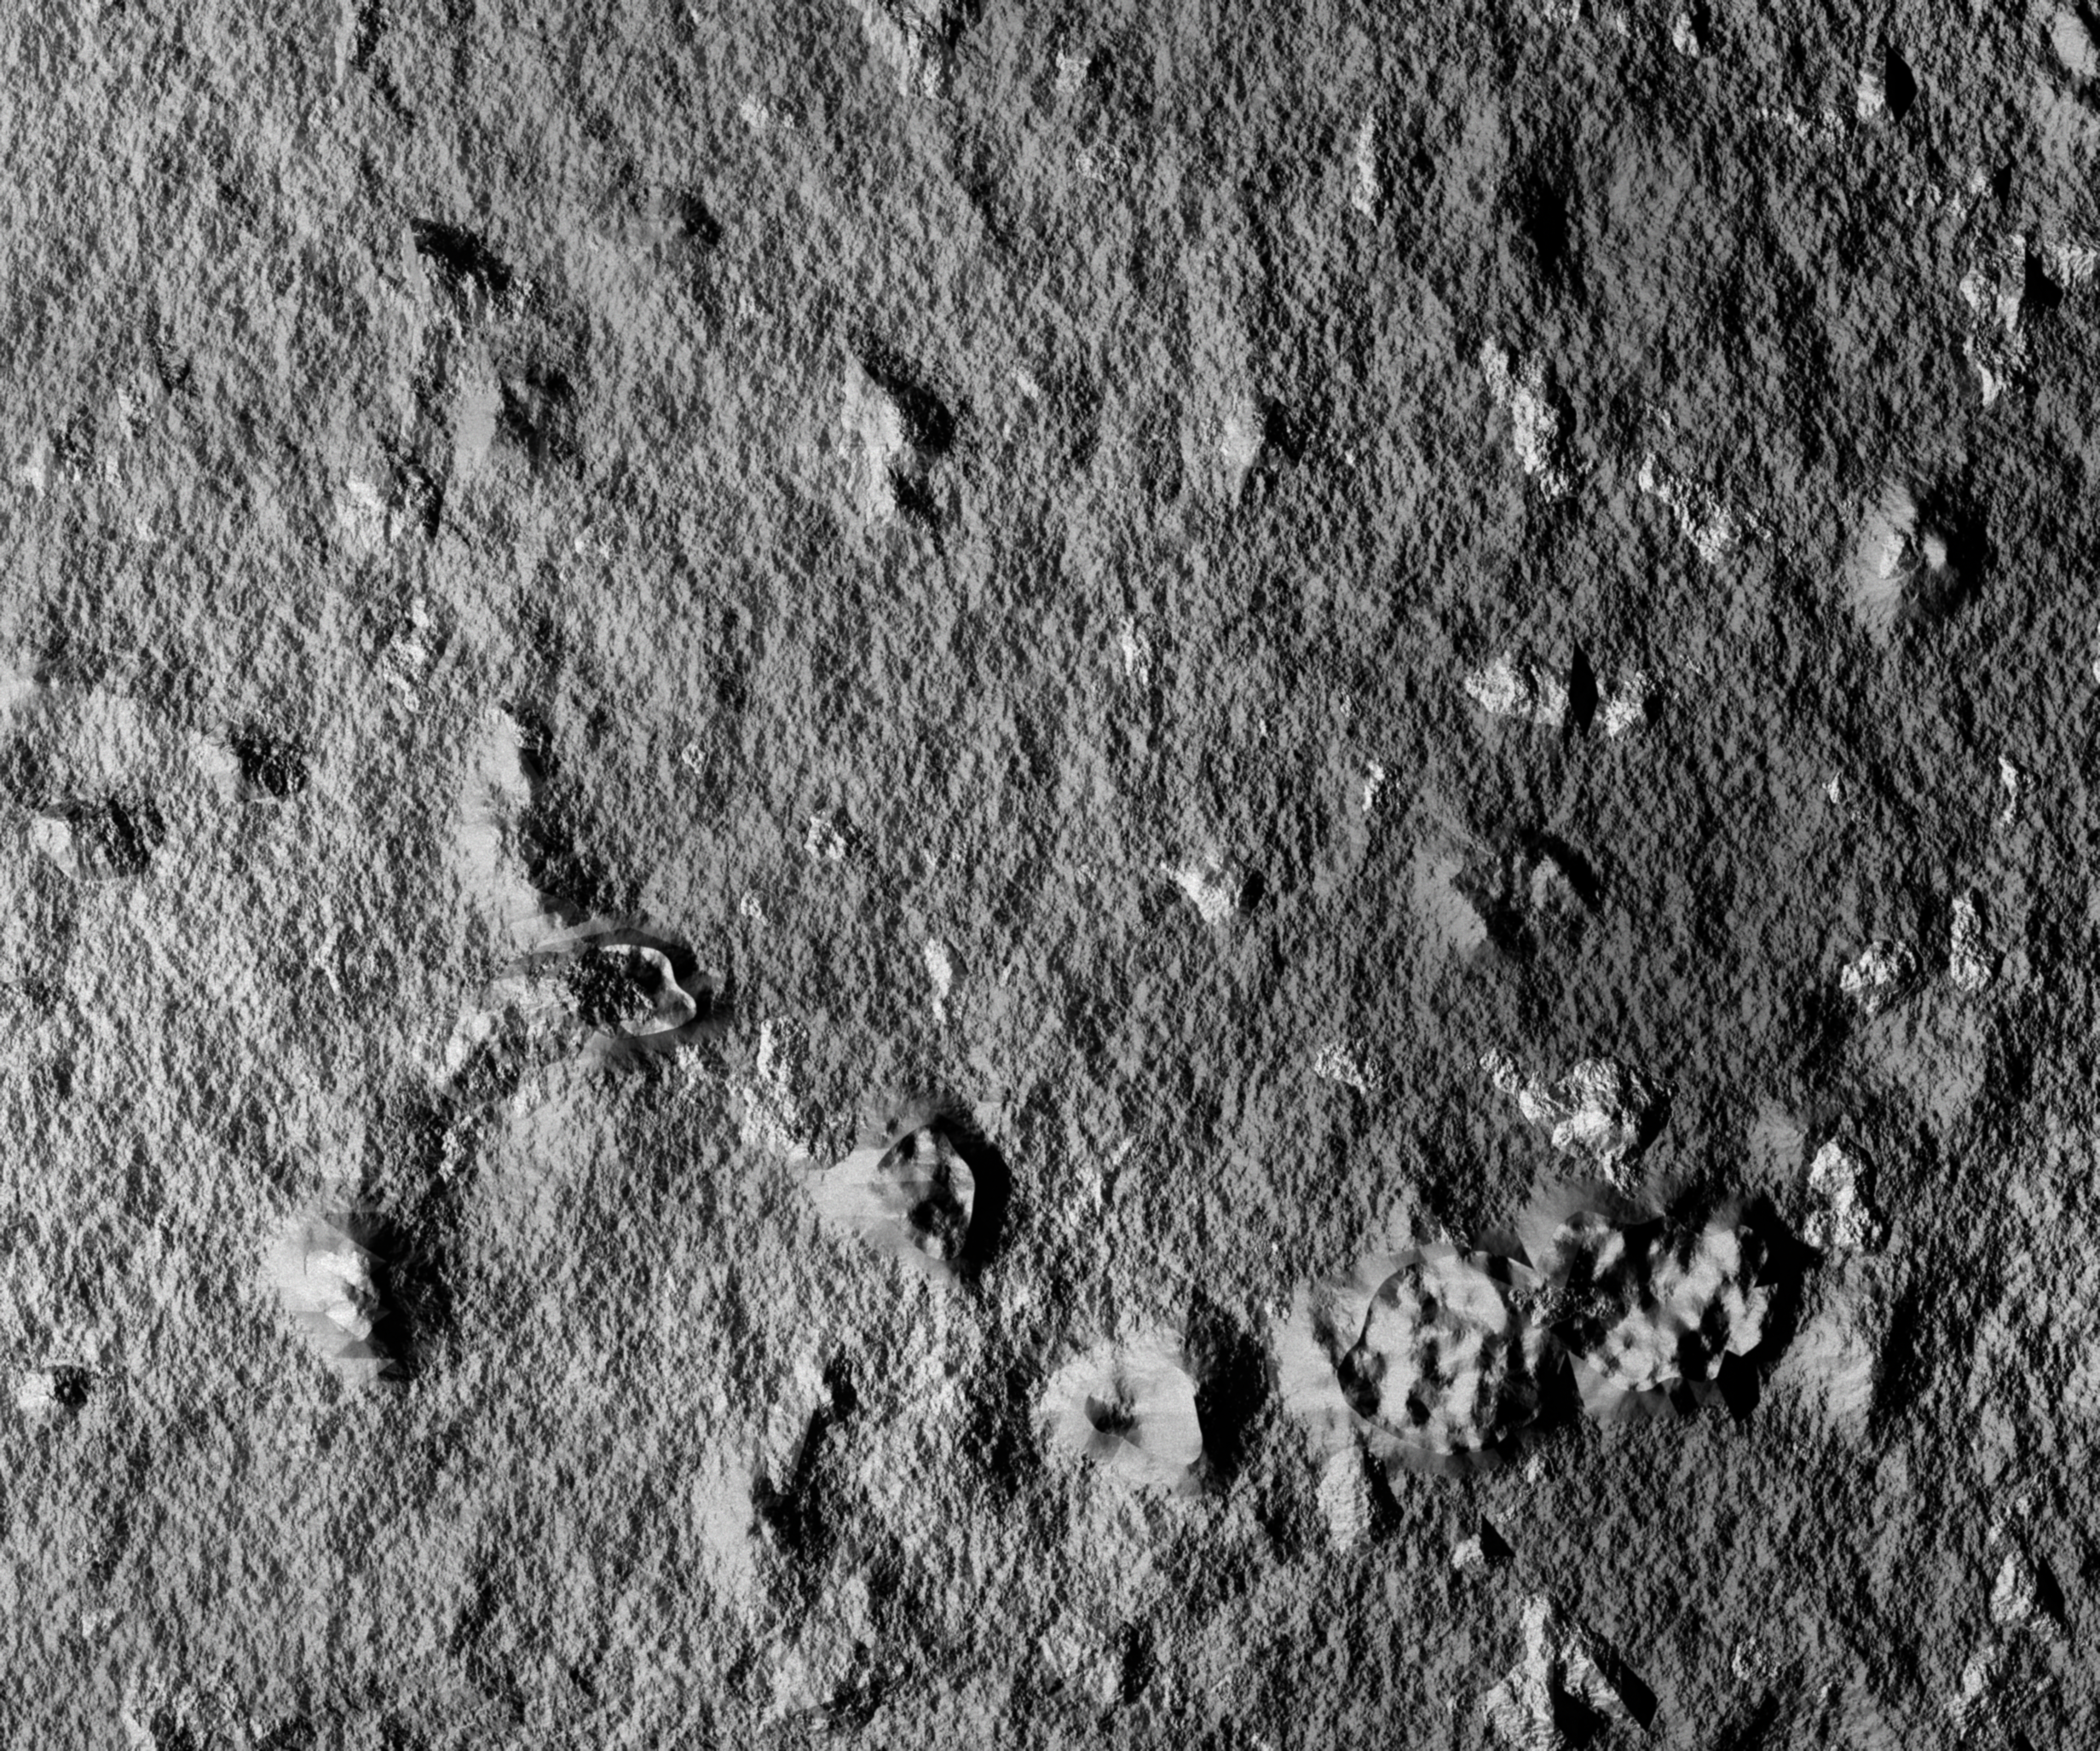
\includegraphics[width=\textwidth]{doc/thesis/0_figures/procedural_terrain/50_10_Inst_2017-08-15T115855-260000.png}
        \caption{}
        \label{fig:render_quali_comparison_2}
    \end{subfigure}
    \\
    \begin{subfigure}[b]{0.48\textwidth}
        \centering
        \includegraphics[width=\textwidth]{doc/thesis/0_figures/procedural_terrain/50_1_Inst_2017-08-15T115837-133000.png}
        \caption{}
        \label{fig:render_quali_comparison_3}
    \end{subfigure}
    \begin{subfigure}[b]{0.48\textwidth}
        \centering
        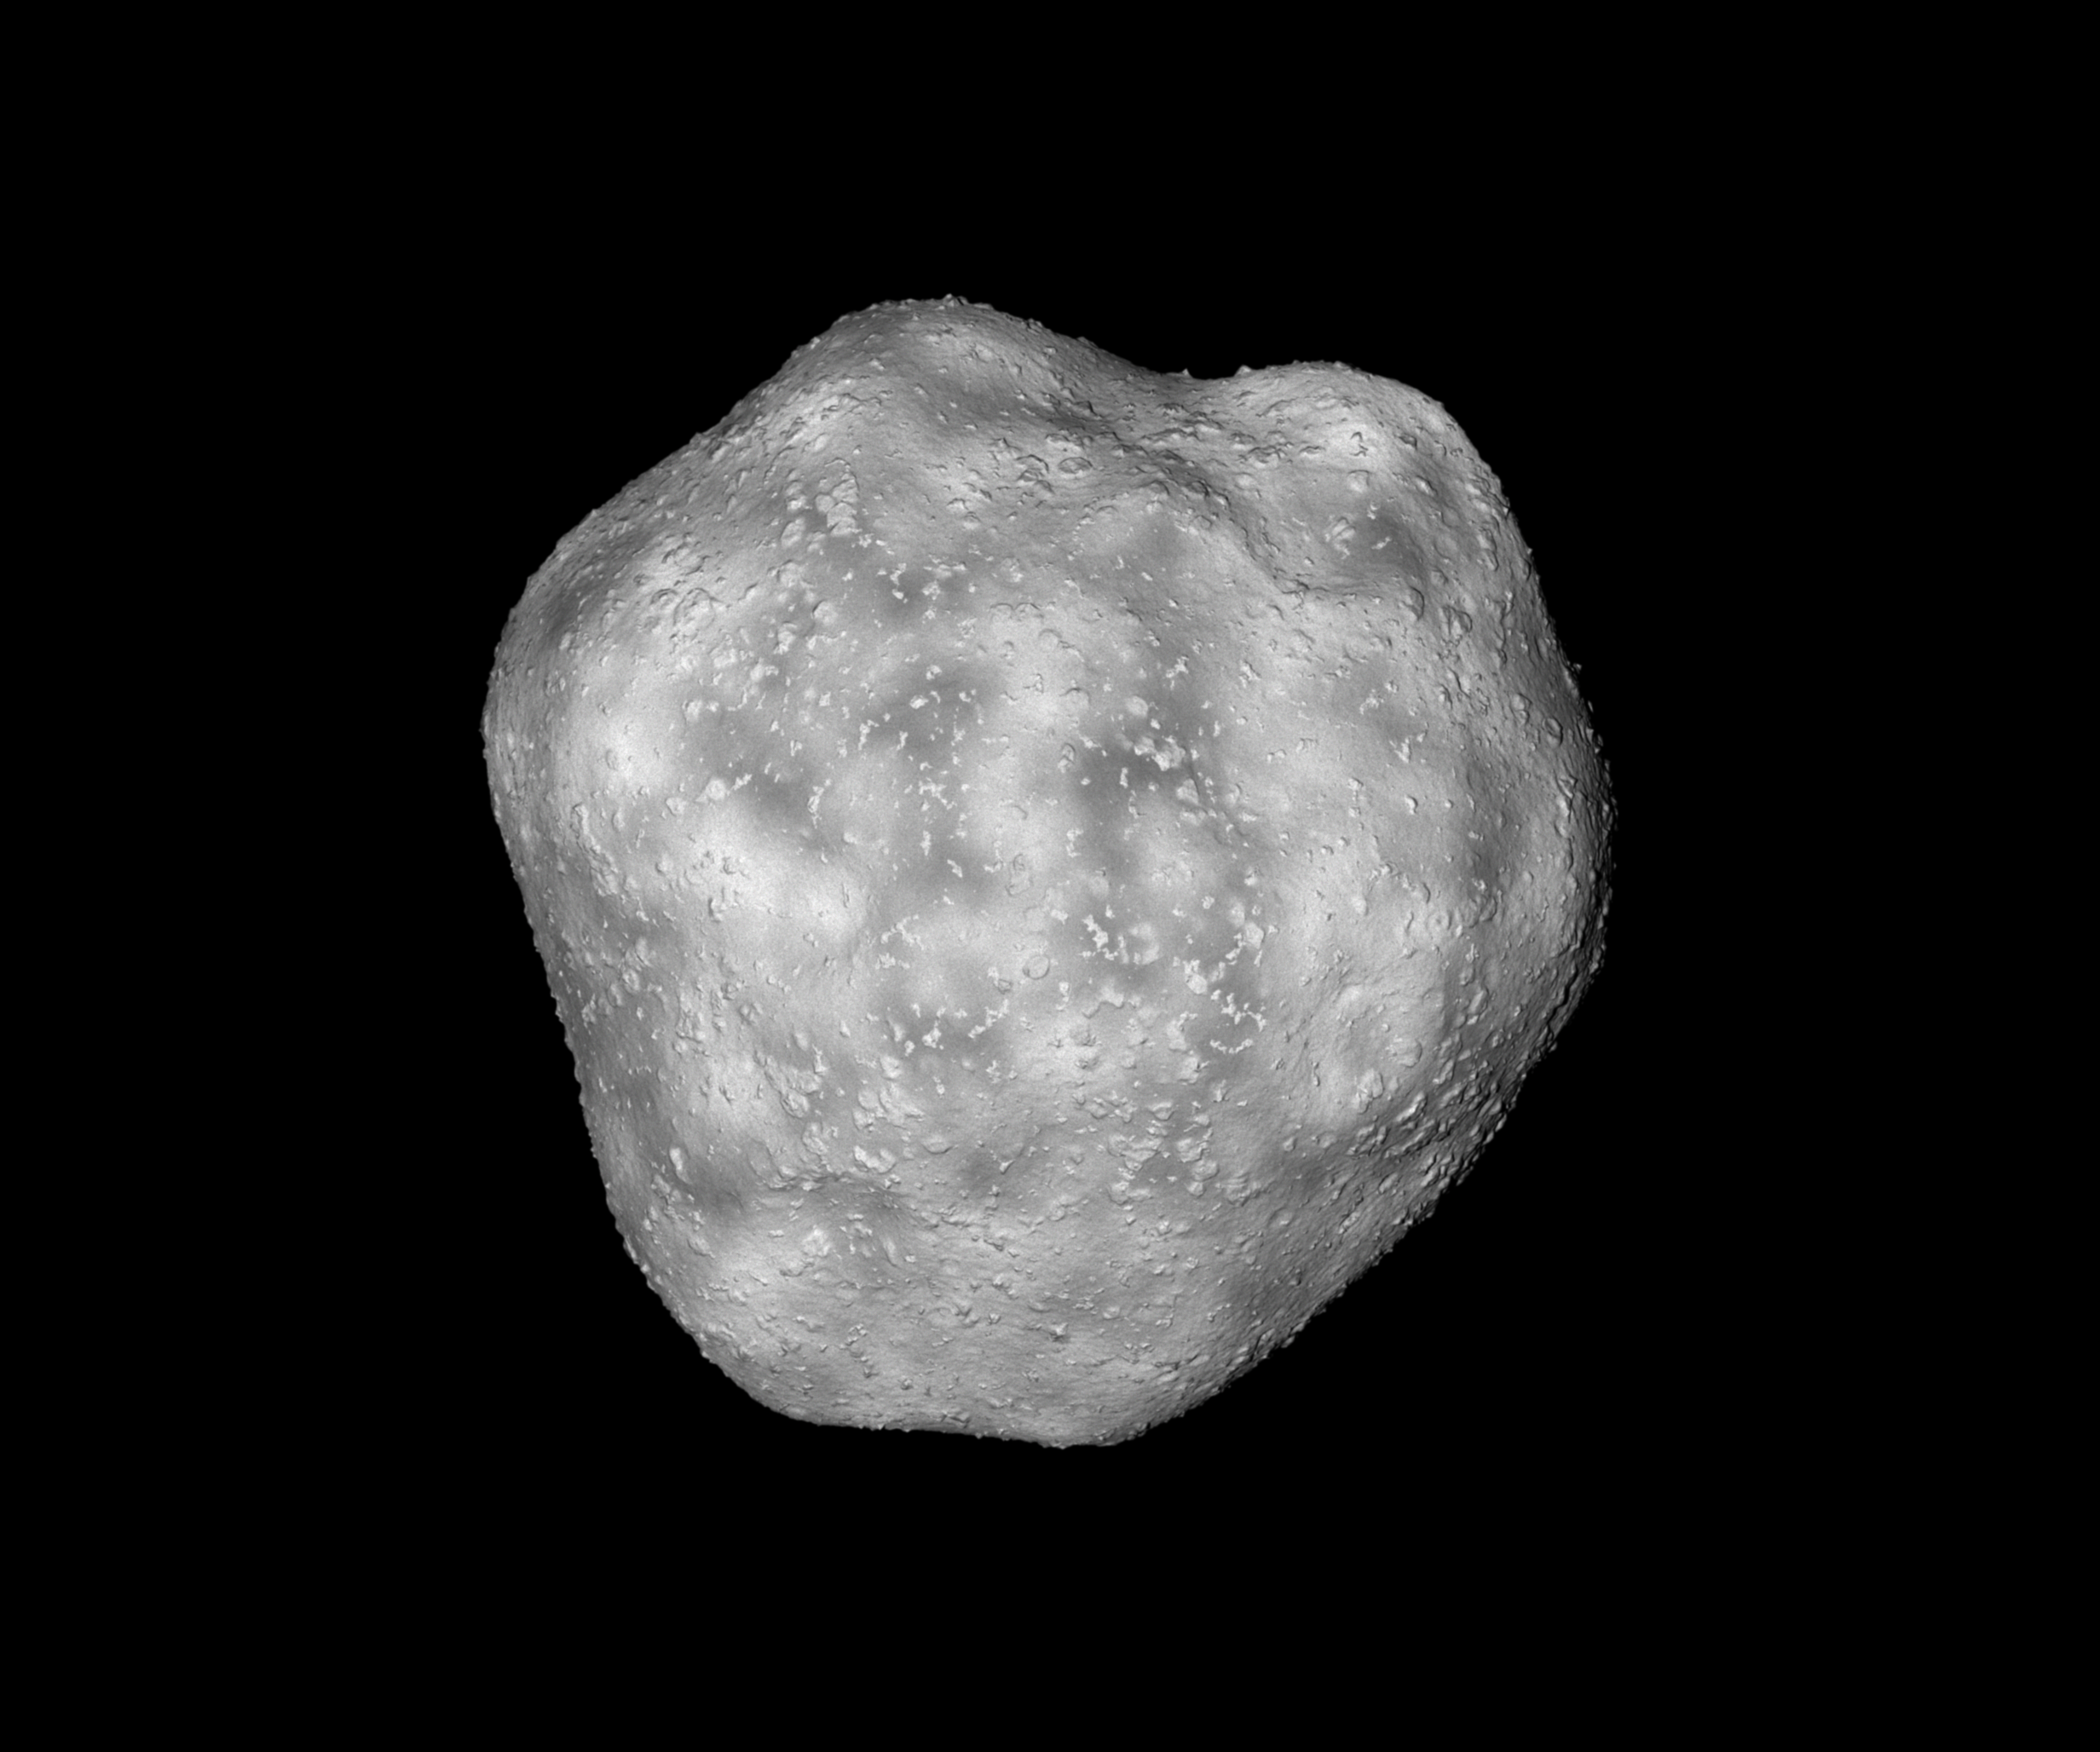
\includegraphics[width=\textwidth]{doc/thesis/0_figures/procedural_terrain/50_1_Inst_2017-08-15T115851-232000.png}
        \caption{}
        \label{fig:render_quali_comparison_4}
    \end{subfigure}
    \caption{Rendered images of an \gls{sssb} nucleus of different sizes from varying distances. (a) Nucleus of \SI{10}{\kilo\meter} from \SI{566}{\kilo\meter} distance. (b) Nucleus of \SI{10}{\kilo\meter} from \SI{106}{\kilo\meter} distance. (c) Nucleus of \SI{1}{\kilo\meter} from \SI{149}{\kilo\meter} distance. (d) Nucleus of \SI{1}{\kilo\meter} from \SI{50}{\kilo\meter} distance.}
    \label{fig:render_quali_comparison}
\end{figure}

\begin{figure}[htb]
    \centering
    \begin{subfigure}[b]{0.59\textwidth}
        \centering
        \includegraphics[width=\textwidth]{doc/thesis/0_figures/procedural_terrain/2963_Bennu.png}
        \caption{}
        \label{fig:render_quali_bennu}
    \end{subfigure} %
    \begin{subfigure}[b]{0.4\textwidth}
        \centering
        \includegraphics[width=\textwidth]{doc/thesis/0_figures/procedural_terrain/67P_CG.PNG}
        \caption{}
        \label{fig:render_quali_67p}
    \end{subfigure}
    \\
    \begin{subfigure}[b]{0.6\textwidth}
        \centering
        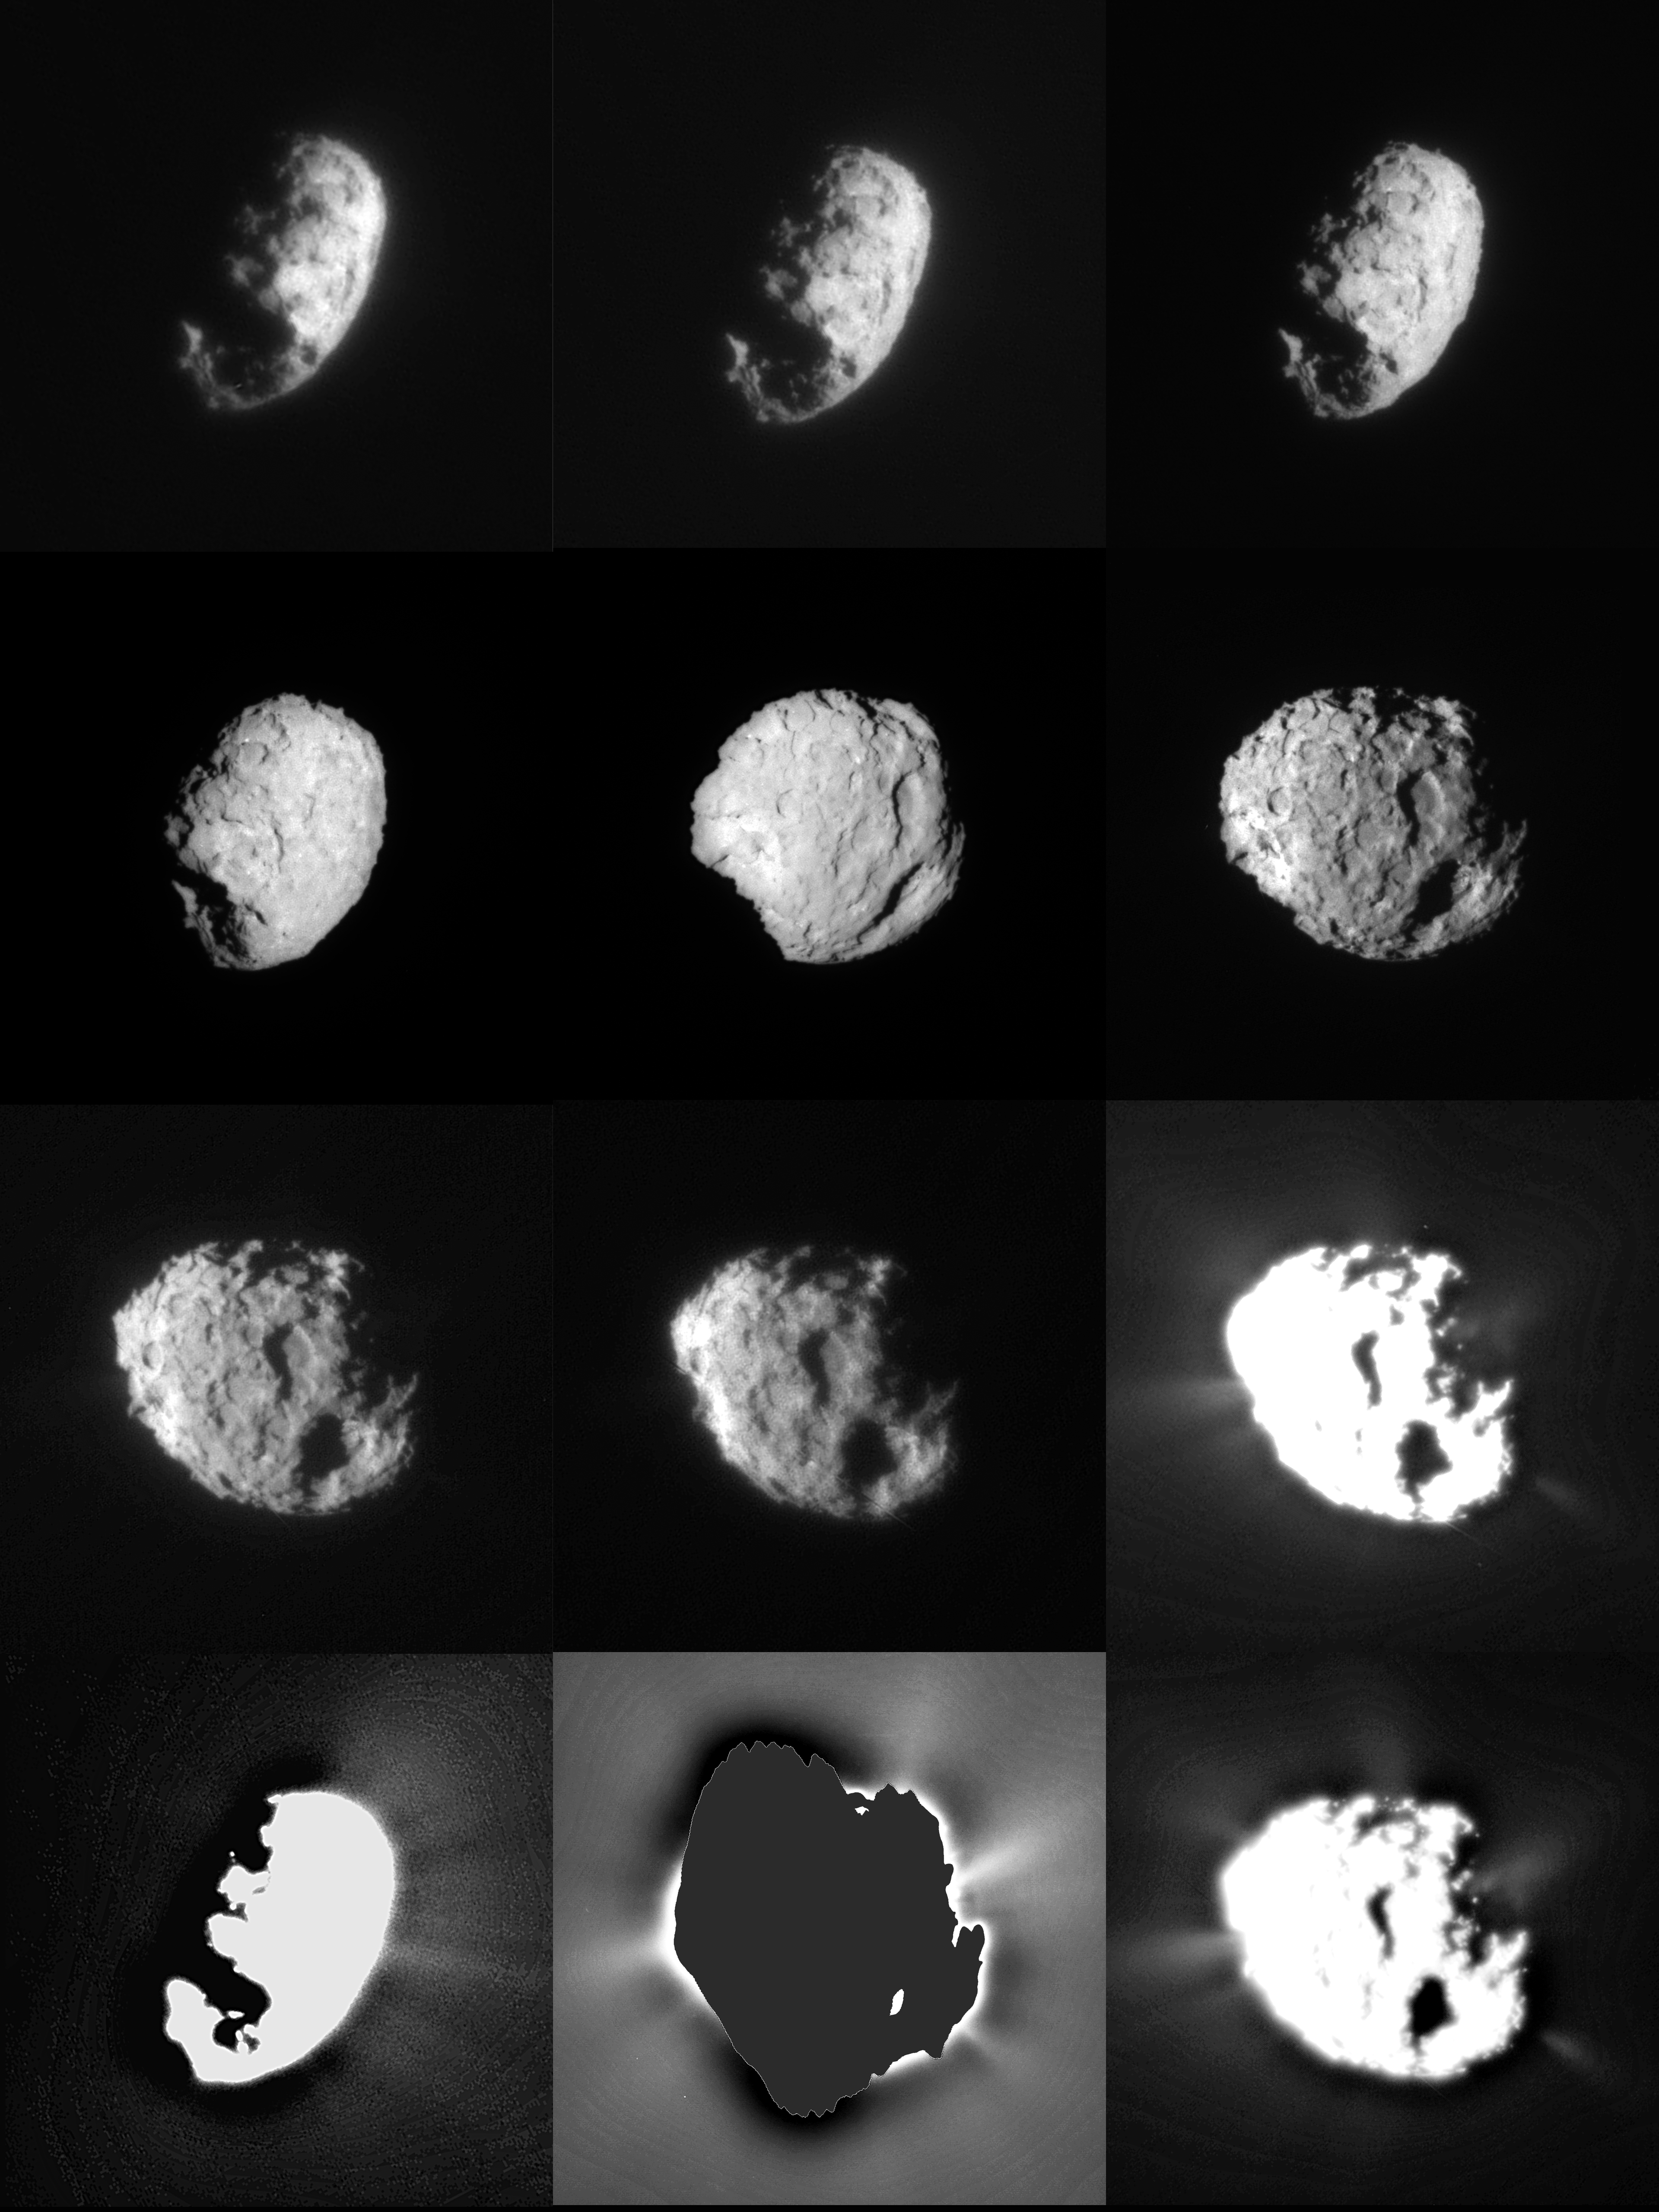
\includegraphics[width=\textwidth]{doc/thesis/0_figures/procedural_terrain/Wild2.jpg}
        \caption{}
        \label{fig:render_quali_81p}
    \end{subfigure}
    \label{fig:render_quali}
    \caption{(a) Four images of asteroid Bennu and a global surface mosaic. These images were taken by the PolyCam aboard the \textit{OSIRIS-REx} mission~\cite{NASAFourBennu}. (b) Representative image of comet \acrlong{67p}. The image was taken by the OSIRIS imager aboard the \textit{Rosetta} mission~\cite{OSIRISArchiveb}. (c) Collection of images of comet \acrlong{81p} taken during the \textit{Stardust} mission by its navigation camera~\cite{StardustImages}.}
\end{figure}

While all images show pits, the overall appearance of the rendered images resembles the smoother pits of Bennu better than the sharper pits of \gls{67p} or \gls{81p}. The overall looks of the rendered images resemble the real images of Bennu well. The rocks and boulders present on Bennu's surface appear similar to the rocks and boulders in the rendered images. When comparing the rendered images to the images of \gls{67p} or \gls{81p}, the most pronounced difference are the jets. \Gls{sispo} does not yet contain a gas and dust model that would produce a coma or jets and therefore these are missing in the rendered images. While the surface of both comets feature some rocks and boulders, there surfaces more defined by ridge-like structures. This type of feature is missing in the rendered images. Hence, the rendering output of \gls{sispo} better represents asteroids than comets.

Through procedural terrain generation, \gls{sispo} produces results for a large range of encounter distances. Example images with different surface distances and \gls{sssb} sizes are shown in Figure~\ref{fig:render_quali_comparison}.It is visible from Figure~\ref{fig:render_quali_comparison} that surface features and details do not degrade visually. Moving closer to the surface reveals more details, such as tiny bumps between larger structures which are not visible from larger distances. The visible quality of surface features is defined by the shader implementation. 

\subsubsection{Image Composition}
The composition process uses raw images rendered with Blender and produces photometrically calibrated images. An example set of four images consisting of two images before and after calibration is shown in Figure~\ref{fig:composition_before_after}. All four images were converted to \SI{8}{\bit} images. Two effects can be seen. First, the original images differ in there overall brightness. This difference is removed by the calibration. Secondly, images become brighter by the calibration process. 

\begin{figure}[htb]
    \centering
    \begin{subfigure}[b]{0.48\textwidth}
        \centering
        \includegraphics[width=\textwidth]{doc/thesis/0_figures/rendering_lighting/SssbOnly_2017-08-15T115858-281000.jpg}
        \caption{}
        \label{fig:composition_before_1}
    \end{subfigure}
    \begin{subfigure}[b]{0.48\textwidth}
        \centering
        \includegraphics[width=\textwidth]{doc/thesis/0_figures/rendering_lighting/SssbOnly_2017-08-15T115859-288000.jpg}
        \caption{}
        \label{fig:composition_before_2}
    \end{subfigure}
    \\
    \begin{subfigure}[b]{0.48\textwidth}
        \centering
        \includegraphics[width=\textwidth]{doc/thesis/0_figures/rendering_lighting/Inst_2017-08-15T115858-281000.png}
        \caption{}
        \label{fig:composition_after_1}
    \end{subfigure}
    \begin{subfigure}[b]{0.48\textwidth}
        \centering
        \includegraphics[width=\textwidth]{doc/thesis/0_figures/rendering_lighting/Inst_2017-08-15T115859-288000.png}
        \caption{}
        \label{fig:composition_after_2}
    \end{subfigure}
    \caption{Two consecutive images before and after the composition process. The nucleus is much brighter than background stars thus no stars are visible in these images after calibration. (a)~Image 1 before calibration. (b)~Image 2 before calibration. (c)~Image 1 after calibration. (d)~Image 2 after calibration.}
    \label{fig:composition_before_after}
\end{figure}

% As Figures~\ref{fig:composition_after_1} and \ref{fig:composition_after_2} show, the composition properly calibrates the overall brightness of different images. However, there are sometimes darker and brighter patches within images that are not yet calibrated properly. Figure 

% \begin{figure}[htb]
%     \centering
%         \begin{subfigure}[b]{0.32\textwidth}
%             \centering
%             \includegraphics[width=\textwidth]{doc/thesis/0_figures/composition_varying_brightness/Inst_2017-08-15T115803-901000.png}
%             \label{fig:composition_varying_1}
%         \end{subfigure}
%         \begin{subfigure}[b]{0.32\textwidth}
%             \centering
%             \includegraphics[width=\textwidth]{doc/thesis/0_figures/composition_varying_brightness/Inst_2017-08-15T115804-908000.png}
%             \label{fig:composition_varying_2}
%         \end{subfigure}
%         \begin{subfigure}[b]{0.32\textwidth}
%             \centering
%             \includegraphics[width=\textwidth]{doc/thesis/0_figures/composition_varying_brightness/Inst_2017-08-15T115805-915000.png}
%             \label{fig:composition_varying_3}
%         \end{subfigure}
%     \caption{Varying brightness of patches on the \gls{sssb} surface.}
%     \label{fig:composition_varying}
% \end{figure}

\subsubsection{Rendering Problems} \label{sec:render_problems}
Rendering a fly-by scenario with a \SI{10}{\kilo\meter} \gls{sssb} created artefacts in the images. Figure~\ref{fig:render_artefacts} shows renders from fly-bys with different closest distances from the nucleus. All three images are the raw output from rendering, before composition. The images show a stripe, a darker patch across the \gls{sssb} with sharp brightness transitions. Moreover, the stripe is at the same location across the \gls{sssb} in all three images. This type of artefact does not appear for other \gls{sssb} sizes and not in all images with a \SI{10}{\kilo\meter} \gls{sssb}. The most likely explanation are errors while scaling the nucleus from the original \SI{1}{\kilo\meter} to the \SI{10}{\kilo\meter} model.
\begin{figure}[htb]
    \centering
    \begin{subfigure}[b]{0.32\textwidth}
        \centering
        \includegraphics[width=\textwidth]{doc/thesis/0_figures/rendering_artefacts/50_10_SssbOnly_2017-08-15T115845-190000.jpg}
        \caption{}
        \label{fig:render_artefacts_50}
    \end{subfigure}
    \begin{subfigure}[b]{0.32\textwidth}
        \centering
        \includegraphics[width=\textwidth]{doc/thesis/0_figures/rendering_artefacts/200_10_SssbOnly_2017-08-15T115845-190000.jpg}
        \caption{}
        \label{fig:render_artefacts_200}
    \end{subfigure}
    \begin{subfigure}[b]{0.32\textwidth}
        \centering
        \includegraphics[width=\textwidth]{doc/thesis/0_figures/rendering_artefacts/400_10_SssbOnly_2017-08-15T115845-190000.jpg}
        \caption{}
        \label{fig:render_artefacts_400}
    \end{subfigure}
    \caption{Surface of a \SI{10}{\kilo\meter} \gls{sssb} for varying fly-by distances. Rendering artefacts, the stripes, are clearly visible in all three images. (a)~Closest-approach \SI{50}{\kilo\meter}. (b)~Closest-approach \SI{200}{\kilo\meter}. (c)~Closest-approach \SI{400}{\kilo\meter}.}
    \label{fig:render_artefacts}
\end{figure}

A second problem occurred in a \SI{50}{\kilo\meter} fly-by simulation with a \SI{1}{\kilo\meter} \gls{sssb}. A single image was found to be darker than all other images in the data set. Figure~\ref{fig:render_dark} shows three images where the middle image is overall darker except for one small patch of white pixels. Three pixels are much brighter than any other pixel in the image. These are so-called \textit{fireflies}~\cite{Valenza2015BlenderCookbook}. Figure~\ref{fig:render_dark} contains composed images for better visibility of the artefact. The artefact is not introduced by the composition process since it exists in the raw rendered images. No second image with the same issue was found in any other data set therefore the problem was not investigated further.

\begin{figure}[htb]
    \centering
        \begin{subfigure}[b]{0.32\textwidth}
            \centering
            \includegraphics[width=\textwidth]{doc/thesis/0_figures/composition_darkening/50km_Inst_2017-08-15T115816-993000_center.png}
            \label{fig:render_dark_1}
        \end{subfigure}
        \begin{subfigure}[b]{0.32\textwidth}
            \centering
            \includegraphics[width=\textwidth]{doc/thesis/0_figures/composition_darkening/Inst_2017-08-15T115818-000000_center.png}
            \label{fig:render_dark_2}
        \end{subfigure}
        \begin{subfigure}[b]{0.32\textwidth}
            \centering
            \includegraphics[width=\textwidth]{doc/thesis/0_figures/composition_darkening/Inst_2017-08-15T115819-007000_center.png}
            \label{fig:render_dark_3}
        \end{subfigure}
    \caption{Overall darkened \gls{sssb} image due to three pixels being much brighter. These pixels are referred to as fireflies. All three images are composed images for better visibility of the artefact. The images are cropped to display the \gls{sssb} nucleus and artefact better.}
    \label{fig:render_dark}
\end{figure}

\clearpage

\subsection{Compression} \label{sec:results_comp}
The \gls{sispo} software package was used to study the effects of compression in different scenarios. The scenarios are presented in Table~\ref{tab:sim_params}. Two compression algorithms were used to study compression effects. The \gls{png} format was used because of its wide support among different software packages and \gls{jp2} is used as an improved version over commonly used \gls{jpeg}. The \gls{png} and \gls{jp2} formats were selected as general examples to characterise the compression effects on reconstruction. Neither of these two algorithms is intended to represent image processing on-board a spacecraft. Scenarios with varying \gls{sssb} nucleus sizes and fly-by distance were simulated. 
Comparison of the different compression algorithms is based on several output parameters. The data size of the compressed image series, the number of points in the dense reconstructed point cloud, the number of vertices and the number of faces of the refined reconstructed model. These outputs relate well to the level of detail of the rendered images, since \gls{sfm} algorithms rely on surface details for reconstruction.

\subsubsection{Image Quality Comparison} \label{sec:img_quali_comp}
To compare the image quality after different levels of compression, a specific image is selected which is compressed to different levels. Since reconstruction is mostly influenced by features, a scene with a distance of \SI{50}{\kilo\meter} was selected for comparison. Once the overall images, containing the entire \gls{sssb} in the \gls{fov}, and closeups, highlighted by the red frame in Figure~\ref{fig:img_quality_frame} are studied. Overall images are used to show compression effects on an entire scene while the closeup images reveal compression effects on surface details. Difference images and histograms are used to further investigate the effects of compression. Difference images are created by converting the \gls{rgb} images to greyscale and taking the L2-norm after subtracting each pixel from the respective value of the \gls{png} greyscale image. The result is a greyscale difference image showing the L2-norm differences. For the histograms, the zero values were removed to only show differences. Therefore, the total number of pixels and the percentage compared to the original that were used for the histogram are given as well.

\begin{figure}[htb]
    \centering
    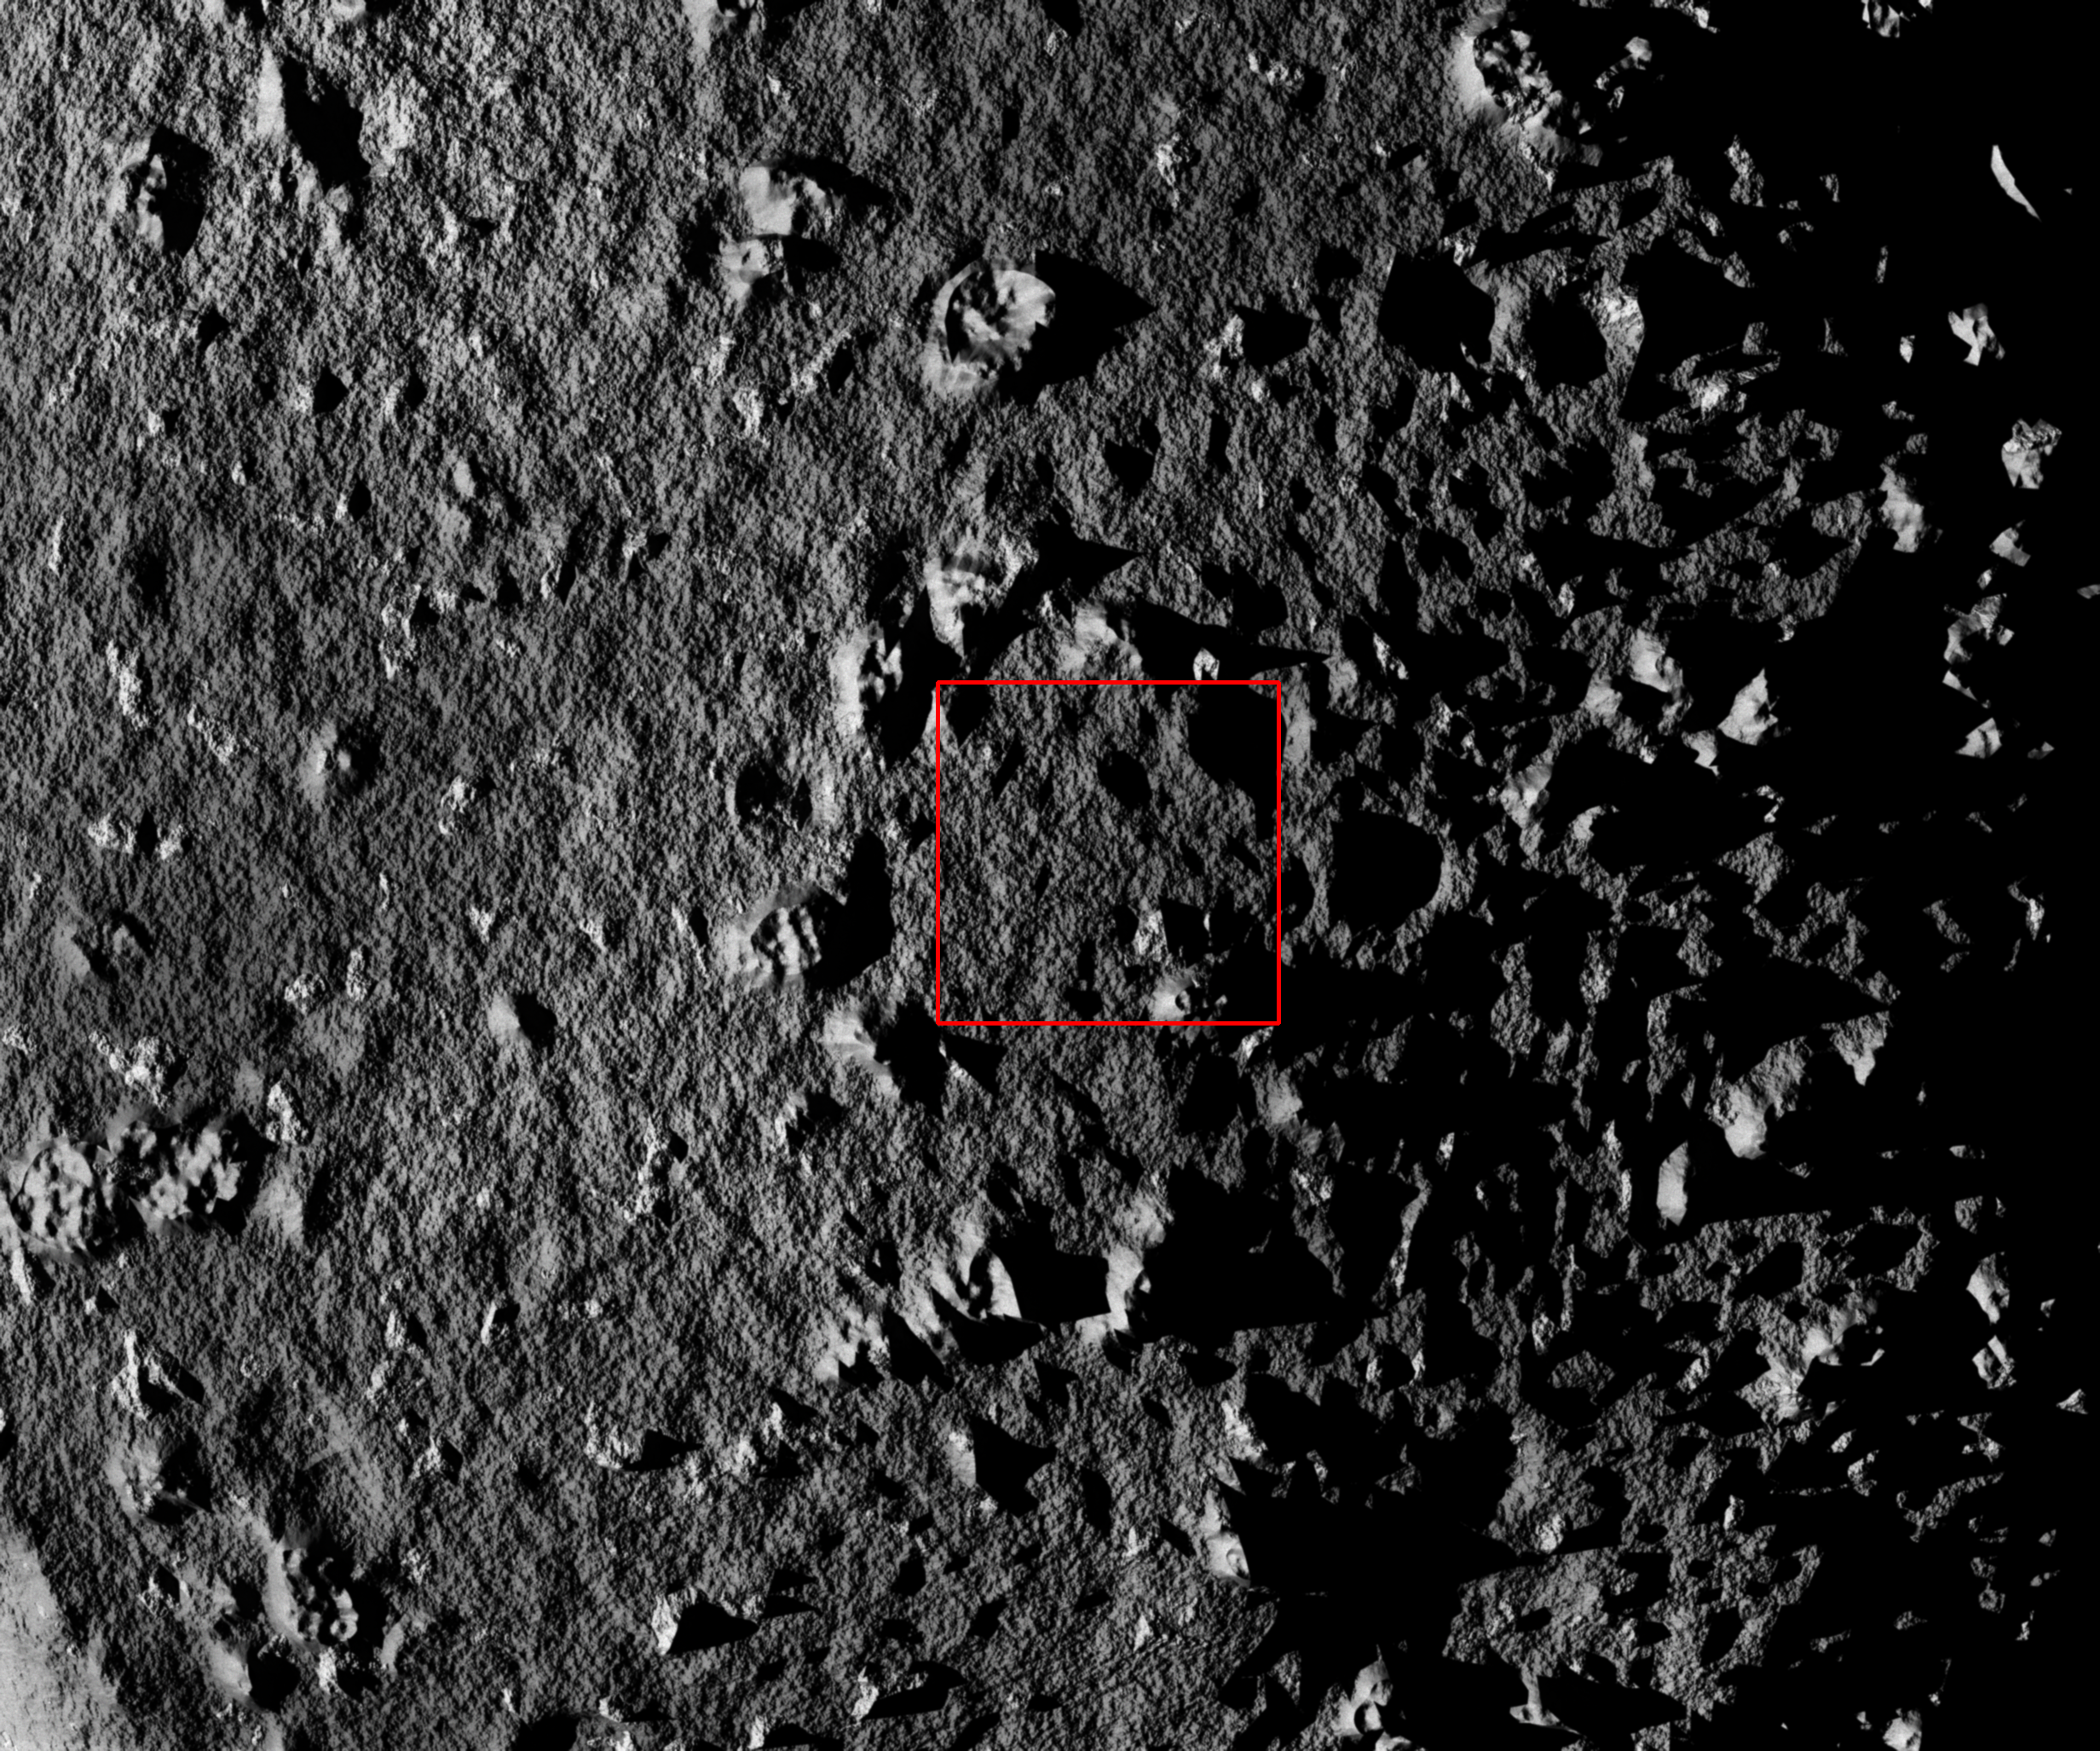
\includegraphics[width=.7\textwidth]{doc/thesis/0_figures/compare_quality/set1/jp2_1000_frame}
    \caption{Scene used for quality comparison. The area highlighted in red is studied up closer. The specific area was selected since it includes a wide range of colours and various sized surface features.}
    \label{fig:img_quality_frame}
\end{figure}

Figures~\ref{fig:img_quality_comp_jp2_1} to \ref{fig:img_quality_comp_jp2_1000} show the compressed overall image, the difference histograms as well as the difference images after compression with \gls{jp2} with quality levels \SI{1}{}, \SI{5}{}, \SI{10}{}, \SI{100}{} and \SI{1000}{}. Quality level \SI{5}{} is used since most changes due to compression occur at low quality levels.

\begin{figure}[htb]
    \centering
    \begin{subfigure}[b]{0.48\textwidth}
        \centering
        \includegraphics[width=\textwidth]{doc/thesis/0_figures/compare_quality/set1/jp2_1}
        \caption{}
        \label{fig:img_quality_comp_jp2_1_orig}
    \end{subfigure}
    \begin{subfigure}[b]{0.48\textwidth}
        \centering
        \includegraphics[width=\textwidth]{doc/thesis/0_figures/compare_quality/set1/jp2_1_diff_histogram}
        \caption{}
        \label{fig:img_quality_comp_jp2_1_histo}
    \end{subfigure}
    \\
    \begin{subfigure}[b]{0.48\textwidth}
        \centering
        \includegraphics[width=\textwidth]{doc/thesis/0_figures/compare_quality/set1/jp2_1_diff_heatmap}
        \caption{}
        \label{fig:img_quality_comp_jp2_1_diff}
    \end{subfigure}
    \begin{subfigure}[b]{0.48\textwidth}
        \centering
        \includegraphics[width=\textwidth]{doc/thesis/0_figures/compare_quality/set1/jp2_1_diff_heatmap_rel}
        \caption{}
        \label{fig:img_quality_comp_jp2_1_diff_rel}
    \end{subfigure}
    \caption{Overall rendered image after compression with \gls{jp2} quality level 1. The L2-norm is applied to the difference between the greyscale images of the lossless and respective lossy image. (a) Image after lossy compression. (b) Histogram of L2-norms of differences. (c) L2-norm difference image with a colour scale from $0$ to $131$ for comparison between various compression levels. (d) L2-norm difference image with a colour scale from $0$ to the maximum L2-norm value for better visibility of compression effects.}
    \label{fig:img_quality_comp_jp2_1}
\end{figure}


\begin{figure}[htb]
    \centering
    \begin{subfigure}[b]{0.48\textwidth}
        \centering
        \includegraphics[width=\textwidth]{doc/thesis/0_figures/compare_quality/set1/jp2_5}
        \caption{}
        \label{fig:img_quality_comp_jp2_5_orig}
    \end{subfigure}
    \begin{subfigure}[b]{0.48\textwidth}
        \centering
        \includegraphics[width=\textwidth]{doc/thesis/0_figures/compare_quality/set1/jp2_5_diff_histogram}
        \caption{}
        \label{fig:img_quality_comp_jp2_5_histo}
    \end{subfigure}
    \\
    \begin{subfigure}[b]{0.48\textwidth}
        \centering
        \includegraphics[width=\textwidth]{doc/thesis/0_figures/compare_quality/set1/jp2_5_diff_heatmap}
        \caption{}
        \label{fig:img_quality_comp_jp2_5_diff}
    \end{subfigure}
    \begin{subfigure}[b]{0.48\textwidth}
        \centering
        \includegraphics[width=\textwidth]{doc/thesis/0_figures/compare_quality/set1/jp2_5_diff_heatmap_rel}
        \caption{}
        \label{fig:img_quality_comp_jp2_5_diff_rel}
    \end{subfigure}
    \caption{Overall rendered image after compression with \gls{jp2} quality level 5. The L2-norm is applied to the difference between the greyscale images of the lossless and respective lossy image. (a) Image after lossy compression. (b) Histogram of L2-norms of differences. (c) L2-norm difference image with a colour scale from $0$ to $131$ for comparison between various compression levels. (d) L2-norm difference image with a colour scale from $0$ to the maximum L2-norm value for better visibility of compression effects.}
    \label{fig:img_quality_comp_jp2_5}
\end{figure}


\begin{figure}[htb]
    \centering
    \begin{subfigure}[b]{0.48\textwidth}
        \centering
        \includegraphics[width=\textwidth]{doc/thesis/0_figures/compare_quality/set1/jp2_10}
        \caption{}
        \label{fig:img_quality_comp_jp2_10_orig}
    \end{subfigure}
    \begin{subfigure}[b]{0.48\textwidth}
        \centering
        \includegraphics[width=\textwidth]{doc/thesis/0_figures/compare_quality/set1/jp2_10_diff_histogram}
        \caption{}
        \label{fig:img_quality_comp_jp2_10_histo}
    \end{subfigure}
    \\
    \begin{subfigure}[b]{0.48\textwidth}
        \centering
        \includegraphics[width=\textwidth]{doc/thesis/0_figures/compare_quality/set1/jp2_10_diff_heatmap}
        \caption{}
        \label{fig:img_quality_comp_jp2_10_diff}
    \end{subfigure}
    \begin{subfigure}[b]{0.48\textwidth}
        \centering
        \includegraphics[width=\textwidth]{doc/thesis/0_figures/compare_quality/set1/jp2_10_diff_heatmap_rel}
        \caption{}
        \label{fig:img_quality_comp_jp2_10_diff_rel}
    \end{subfigure}
    \caption{Overall rendered image after compression with \gls{jp2} quality level 10. The L2-norm is applied to the difference between the greyscale images of the lossless and respective lossy image. (a) Image after lossy compression. (b) Histogram of L2-norms of differences. (c) L2-norm difference image with a colour scale from $0$ to $131$ for comparison between various compression levels. (d) L2-norm difference image with a colour scale from $0$ to the maximum L2-norm value for better visibility of compression effects.}
    \label{fig:img_quality_comp_jp2_10}
\end{figure}

\begin{figure}[htb]
    \centering
    \begin{subfigure}[b]{0.48\textwidth}
        \centering
        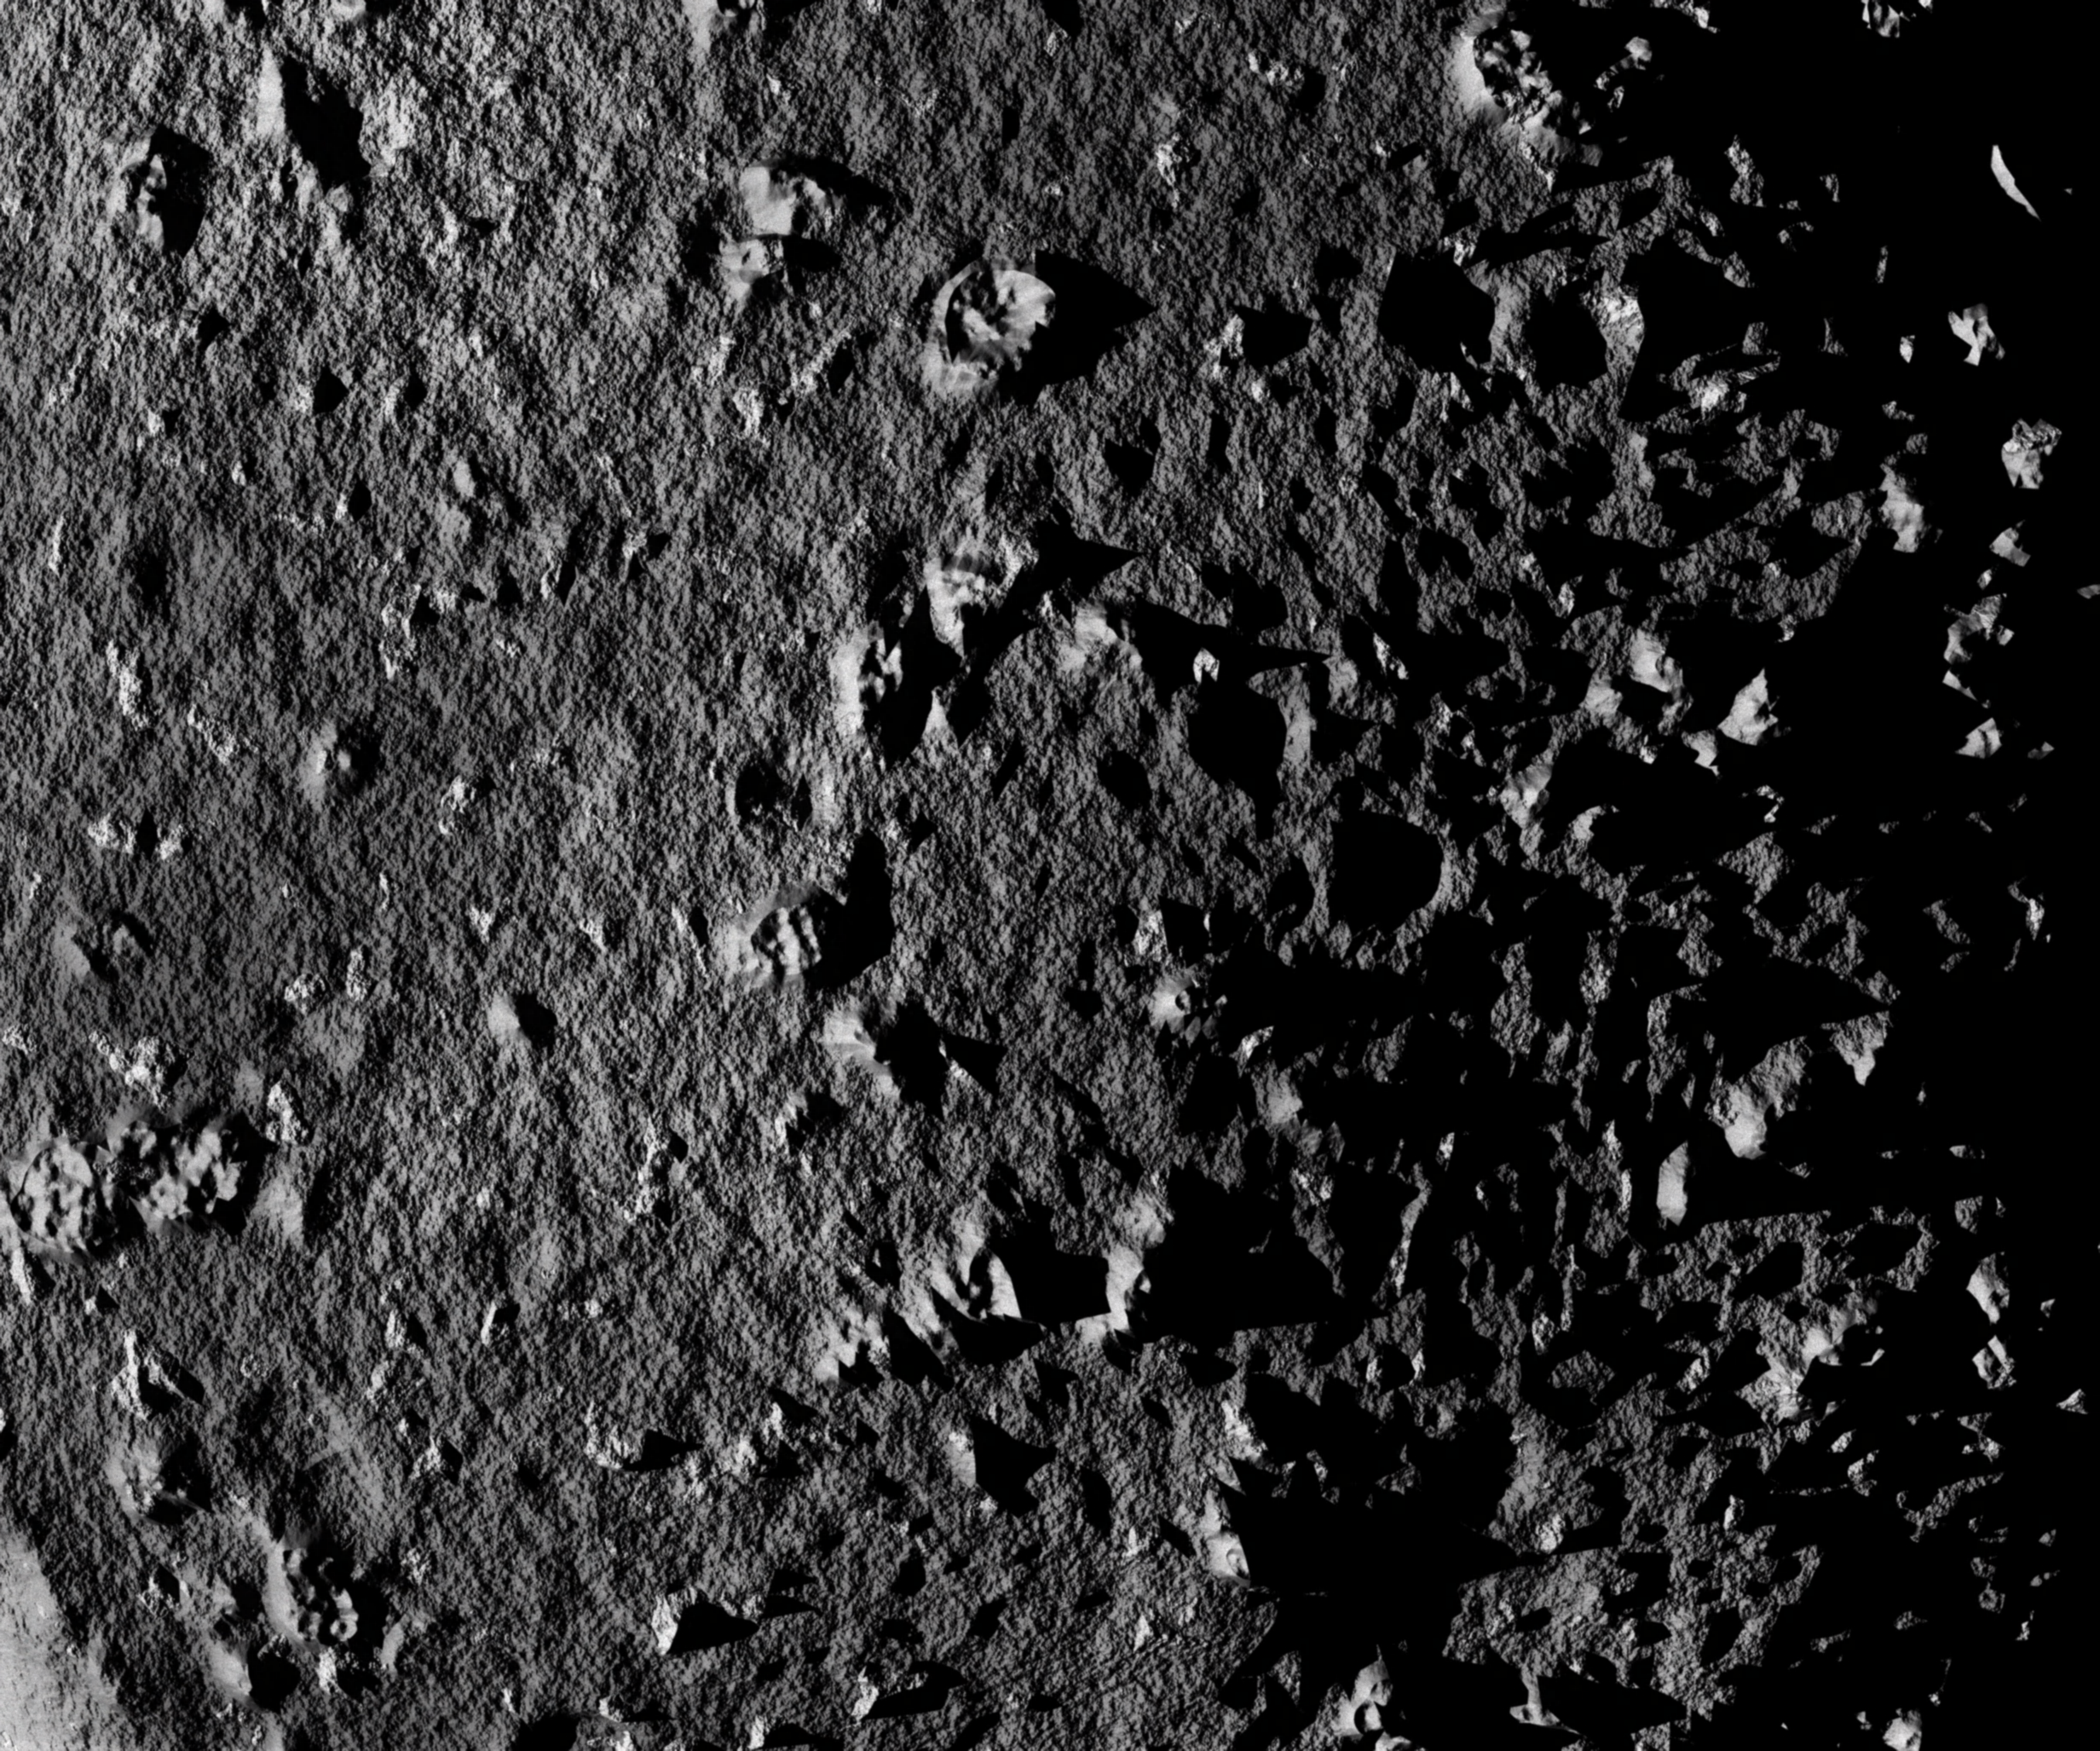
\includegraphics[width=\textwidth]{doc/thesis/0_figures/compare_quality/set1/jp2_100}
        \caption{}
        \label{fig:img_quality_comp_jp2_100_orig}
    \end{subfigure}
    \begin{subfigure}[b]{0.48\textwidth}
        \centering
        \includegraphics[width=\textwidth]{doc/thesis/0_figures/compare_quality/set1/jp2_100_diff_histogram}
        \caption{}
        \label{fig:img_quality_comp_jp2_100_histo}
    \end{subfigure}
    \\
    \begin{subfigure}[b]{0.48\textwidth}
        \centering
        \includegraphics[width=\textwidth]{doc/thesis/0_figures/compare_quality/set1/jp2_100_diff_heatmap}
        \caption{}
        \label{fig:img_quality_comp_jp2_100_diff}
    \end{subfigure}
    \begin{subfigure}[b]{0.48\textwidth}
        \centering
        \includegraphics[width=\textwidth]{doc/thesis/0_figures/compare_quality/set1/jp2_100_diff_heatmap_rel}
        \caption{}
        \label{fig:img_quality_comp_jp2_100_diff_rel}
    \end{subfigure}
    \caption{Overall rendered image after compression with \gls{jp2} quality level 100. The L2-norm is applied to the difference between the greyscale images of the lossless and respective lossy image. (a) Image after lossy compression. (b) Histogram of L2-norms of differences. (c) L2-norm difference image with a colour scale from $0$ to $131$ for comparison between various compression levels. (d) L2-norm difference image with a colour scale from $0$ to the maximum L2-norm value for better visibility of compression effects.}
    \label{fig:img_quality_comp_jp2_100}
\end{figure}

\begin{figure}[htb]
    \centering
    \begin{subfigure}[b]{0.48\textwidth}
        \centering
        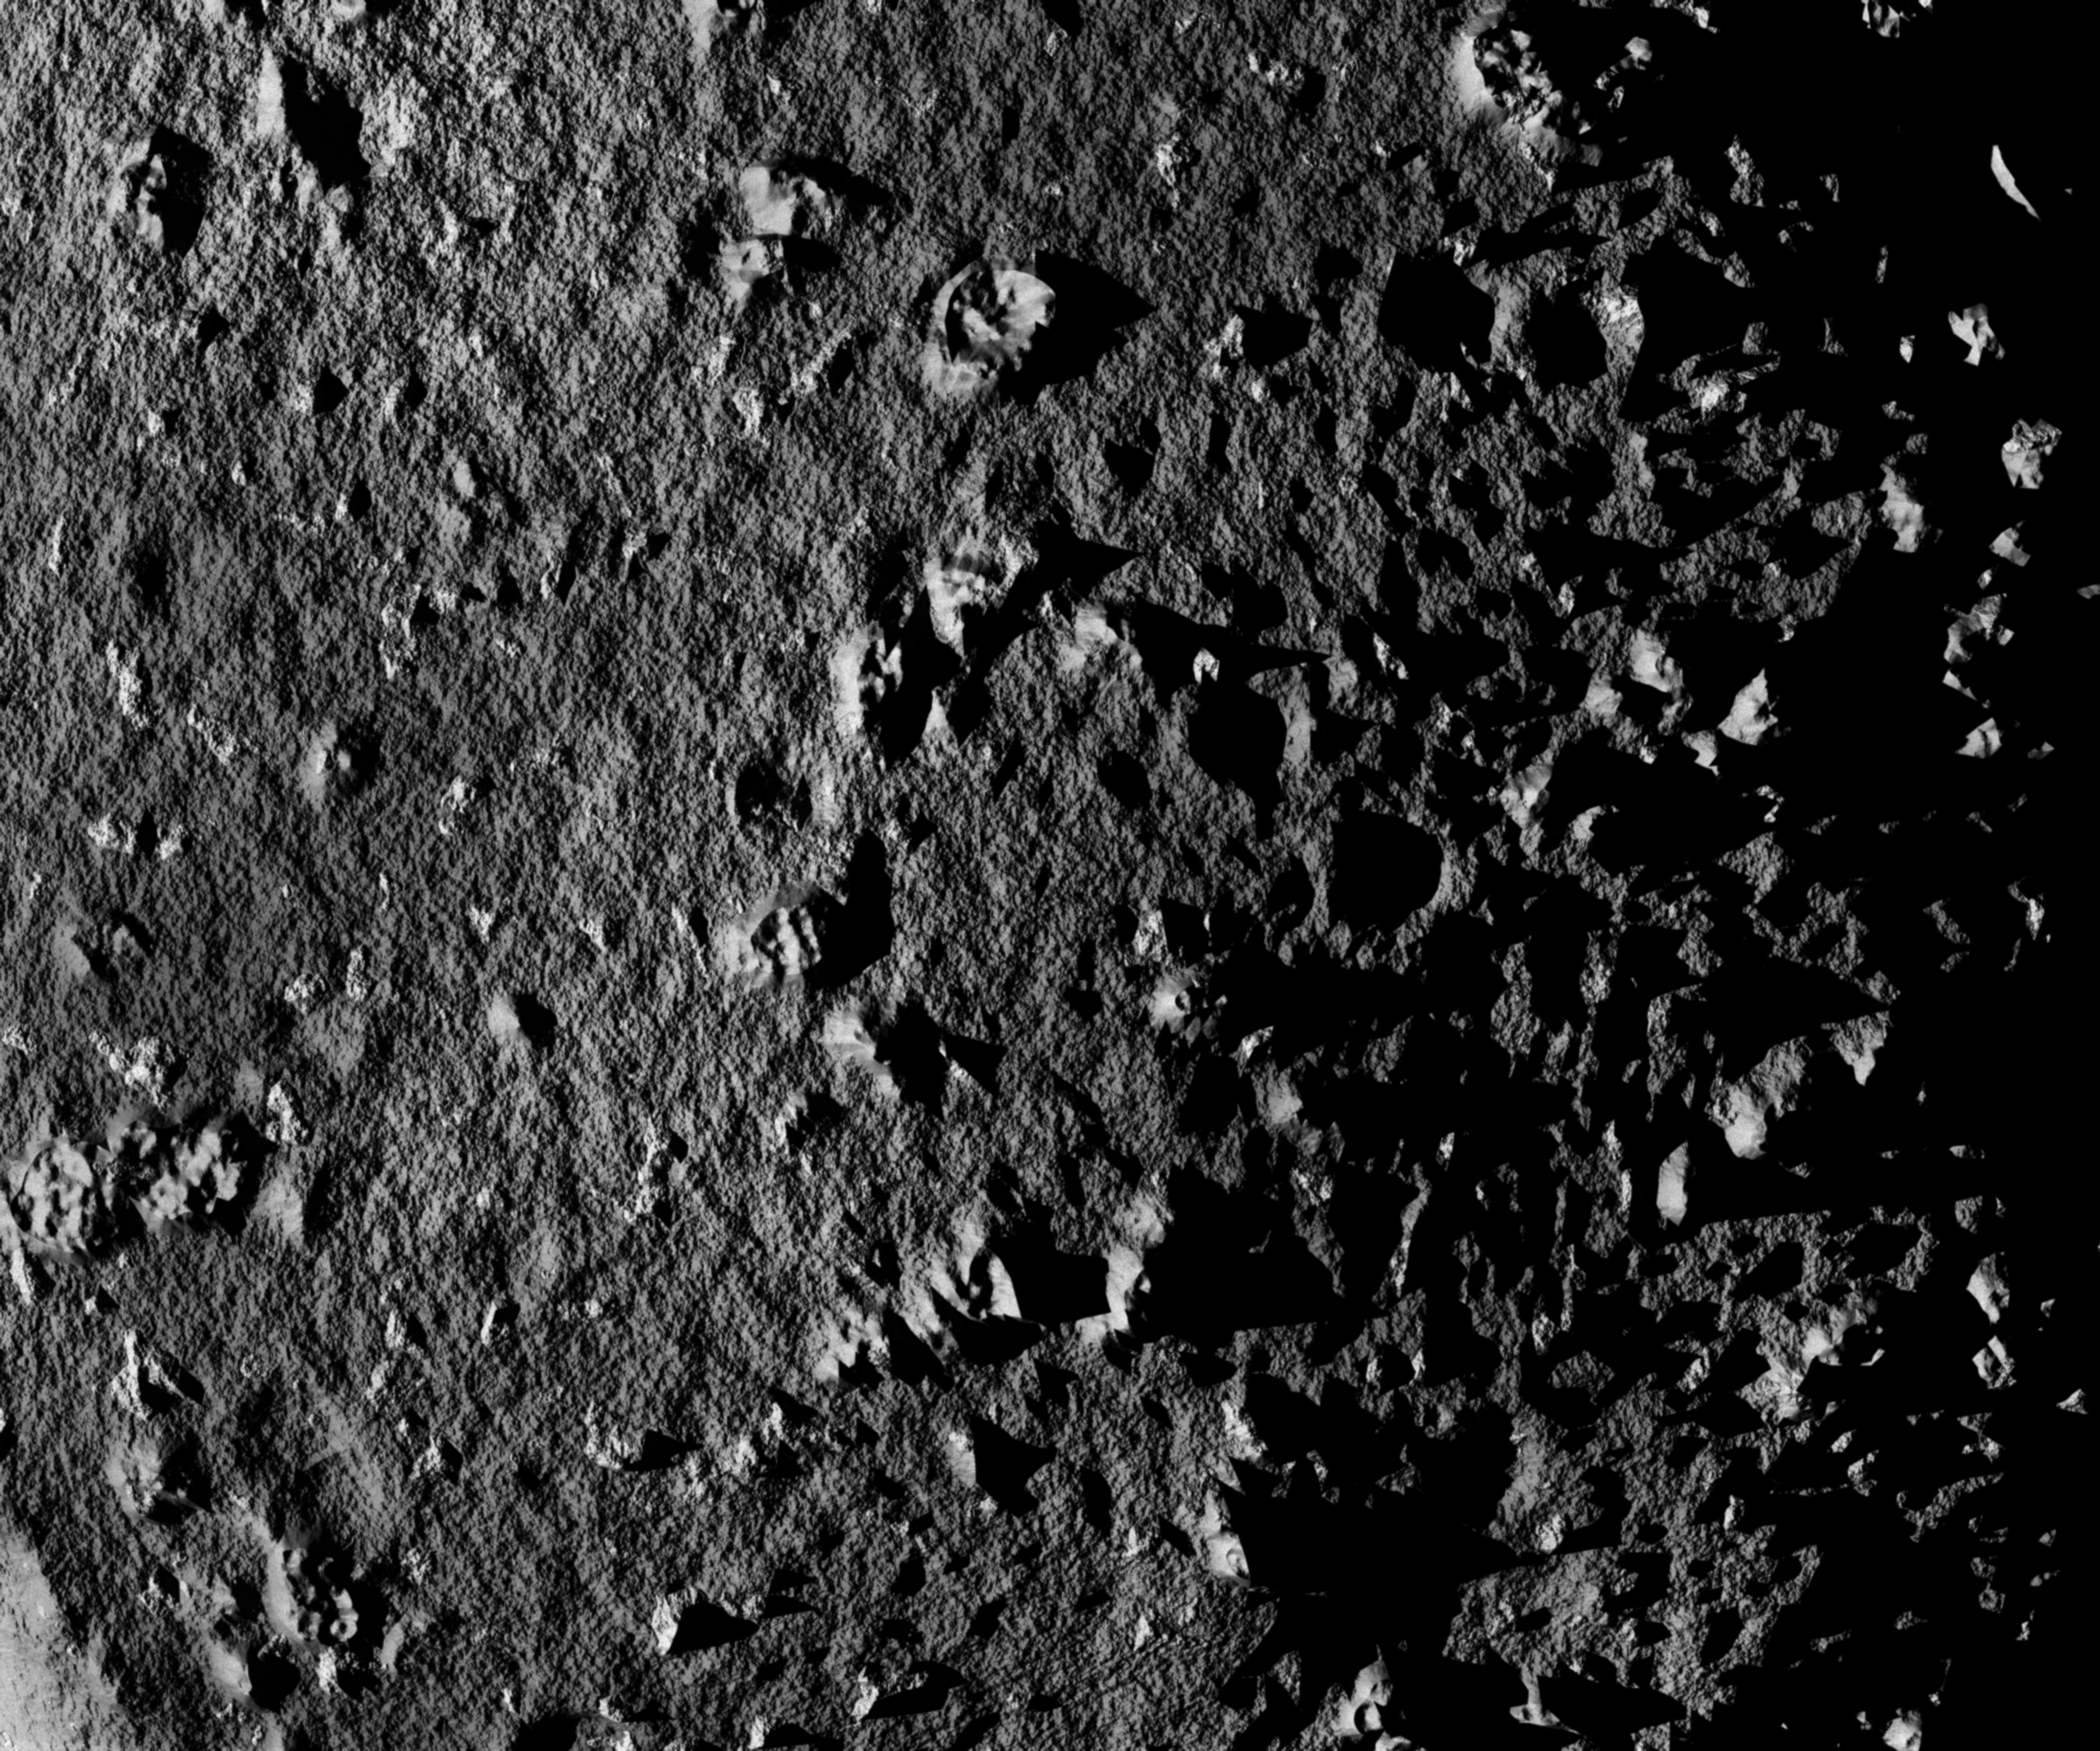
\includegraphics[width=\textwidth]{doc/thesis/0_figures/compare_quality/set1/jp2_1000}
        \caption{}
        \label{fig:img_quality_comp_jp2_1000_orig}
    \end{subfigure}
    \begin{subfigure}[b]{0.48\textwidth}
        \centering
        \includegraphics[width=\textwidth]{doc/thesis/0_figures/compare_quality/set1/jp2_1000_diff_histogram}
        \caption{}
        \label{fig:img_quality_comp_jp2_1000_histo}
    \end{subfigure}
    \\
    \begin{subfigure}[b]{0.48\textwidth}
        \centering
        \includegraphics[width=\textwidth]{doc/thesis/0_figures/compare_quality/set1/jp2_1000_diff_heatmap}
        \caption{}
        \label{fig:img_quality_comp_jp2_1000_diff}
    \end{subfigure}
    \begin{subfigure}[b]{0.48\textwidth}
        \centering
        \includegraphics[width=\textwidth]{doc/thesis/0_figures/compare_quality/set1/jp2_1000_diff_heatmap_rel}
        \caption{}
        \label{fig:img_quality_comp_jp2_1000_diff_rel}
    \end{subfigure}
    \caption{Overall rendered image after compression with \gls{jp2} quality level 1000. The L2-norm is applied to the difference between the greyscale images of the lossless and respective lossy image. (a) Image after lossy compression. (b) Histogram of L2-norms of differences. (c) L2-norm difference image with a colour scale from $0$ to $131$ for comparison between various compression levels. (d) L2-norm difference image with a colour scale from $0$ to the maximum L2-norm value for better visibility of compression effects.}
    \label{fig:img_quality_comp_jp2_1000}
\end{figure}

Overall images show that lossy compression introduces artefacts for all quality levels. Visual inspection of the rendered images does not reveal many changes between different quality levels. However, the histograms reveal that the number of altered pixels and the amount of alteration increases with decreasing quality level. The difference image for quality level 1000 in Figure~\ref{fig:img_quality_comp_jp2_1000_diff_rel} shows the minute changes from compression. The difference images in Figures~\ref{fig:img_quality_comp_jp2_1_diff_rel}, Figure~\ref{fig:img_quality_comp_jp2_5_diff_rel}, Figure~\ref{fig:img_quality_comp_jp2_10_diff_rel} and Figure~\ref{fig:img_quality_comp_jp2_100_diff_rel} outline the shape of the \gls{sssb} showing that compression artefacts are spread across the entire \gls{sssb}. However, when comparing the difference images in Figures~\ref{fig:img_quality_comp_jp2_1_diff}, \ref{fig:img_quality_comp_jp2_5_diff}, \ref{fig:img_quality_comp_jp2_10_diff}, \ref{fig:img_quality_comp_jp2_100_diff} and \ref{fig:img_quality_comp_jp2_1000_diff} which use the same scale for all quality levels, we see the alteration in quality levels \SI{100}{} and \SI{1000}{} are much lower compared to quality levels \SI{1}{}, \SI{5}{} and \SI{10}{}.

Figures~\ref{fig:img_quality_comp_jp2_1_center} to \ref{fig:img_quality_comp_jp2_1000_center} show the compressed closeup image, the difference histograms as well as the difference images after compression with \gls{jp2} with quality levels \SI{1}{}, \SI{5}{}, \SI{10}{}, \SI{100}{} and \SI{1000}{}.

\begin{figure}[htb]
    \centering
    \begin{subfigure}[b]{0.48\textwidth}
        \centering
        \includegraphics[width=\textwidth]{doc/thesis/0_figures/compare_quality/set1/jp2_1_center}
        \caption{}
        \label{fig:img_quality_comp_jp2_1_center_orig}
    \end{subfigure}
    \begin{subfigure}[b]{0.48\textwidth}
        \centering
        \includegraphics[width=\textwidth]{doc/thesis/0_figures/compare_quality/set1/jp2_1_center_diff_histogram}
        \caption{}
        \label{fig:img_quality_comp_jp2_1_center_histo}
    \end{subfigure}
    \\
    \begin{subfigure}[b]{0.48\textwidth}
        \centering
        \includegraphics[width=\textwidth]{doc/thesis/0_figures/compare_quality/set1/jp2_1_center_diff_heatmap}
        \caption{}
        \label{fig:img_quality_comp_jp2_1_center_diff}
    \end{subfigure}
    \begin{subfigure}[b]{0.48\textwidth}
        \centering
        \includegraphics[width=\textwidth]{doc/thesis/0_figures/compare_quality/set1/jp2_1_center_diff_heatmap_rel}
        \caption{}
        \label{fig:img_quality_comp_jp2_1_center_diff_rel}
    \end{subfigure}
    \caption{Close-up rendered image after compression with \gls{jp2} quality level 1. The L2-norm is applied to the difference between the greyscale images of the lossless and respective lossy image. (a) Image after lossy compression. (b) Histogram of L2-norms of differences. (c) L2-norm difference image with a colour scale from $0$ to $131$ for comparison between various compression levels. (d) L2-norm difference image with a colour scale from $0$ to the maximum L2-norm value for better visibility of compression effects.}
    \label{fig:img_quality_comp_jp2_1_center}
\end{figure}

\begin{figure}[htb]
    \centering
    \begin{subfigure}[b]{0.48\textwidth}
        \centering
        \includegraphics[width=\textwidth]{doc/thesis/0_figures/compare_quality/set1/jp2_5_center}
        \caption{}
        \label{fig:img_quality_comp_jp2_5_center_orig}
    \end{subfigure}
    \begin{subfigure}[b]{0.48\textwidth}
        \centering
        \includegraphics[width=\textwidth]{doc/thesis/0_figures/compare_quality/set1/jp2_5_center_diff_histogram}
        \caption{}
        \label{fig:img_quality_comp_jp2_5_center_histo}
    \end{subfigure}
    \\
    \begin{subfigure}[b]{0.48\textwidth}
        \centering
        \includegraphics[width=\textwidth]{doc/thesis/0_figures/compare_quality/set1/jp2_5_center_diff_heatmap}
        \caption{}
        \label{fig:img_quality_comp_jp2_5_center_diff}
    \end{subfigure}
    \begin{subfigure}[b]{0.48\textwidth}
        \centering
        \includegraphics[width=\textwidth]{doc/thesis/0_figures/compare_quality/set1/jp2_5_center_diff_heatmap_rel}
        \caption{}
        \label{fig:img_quality_comp_jp2_5_center_diff_rel}
    \end{subfigure}
    \caption{Close-up rendered image after compression with \gls{jp2} quality level 5. The L2-norm is applied to the difference between the greyscale images of the lossless and respective lossy image. (a) Image after lossy compression. (b) Histogram of L2-norms of differences. (c) L2-norm difference image with a colour scale from $0$ to $131$ for comparison between various compression levels. (d) L2-norm difference image with a colour scale from $0$ to the maximum L2-norm value for better visibility of compression effects.}
    \label{fig:img_quality_comp_jp2_5_center}
\end{figure}

\begin{figure}[htb]
    \centering
    \begin{subfigure}[b]{0.48\textwidth}
        \centering
        \includegraphics[width=\textwidth]{doc/thesis/0_figures/compare_quality/set1/jp2_10_center}
        \caption{}
        \label{fig:img_quality_comp_jp2_10_center_orig}
    \end{subfigure}
    \begin{subfigure}[b]{0.48\textwidth}
        \centering
        \includegraphics[width=\textwidth]{doc/thesis/0_figures/compare_quality/set1/jp2_10_center_diff_histogram}
        \caption{}
        \label{fig:img_quality_comp_jp2_10_center_histo}
    \end{subfigure}
    \\
    \begin{subfigure}[b]{0.48\textwidth}
        \centering
        \includegraphics[width=\textwidth]{doc/thesis/0_figures/compare_quality/set1/jp2_10_center_diff_heatmap}
        \caption{}
        \label{fig:img_quality_comp_jp2_10_center_diff}
    \end{subfigure}
    \begin{subfigure}[b]{0.48\textwidth}
        \centering
        \includegraphics[width=\textwidth]{doc/thesis/0_figures/compare_quality/set1/jp2_10_center_diff_heatmap_rel}
        \caption{}
        \label{fig:img_quality_comp_jp2_10_center_diff_rel}
    \end{subfigure}
    \caption{Close-up rendered image after compression with \gls{jp2} quality level 10. The L2-norm is applied to the difference between the greyscale images of the lossless and respective lossy image. (a) Image after lossy compression. (b) Histogram of L2-norms of differences. (c) L2-norm difference image with a colour scale from $0$ to $131$ for comparison between various compression levels. (d) L2-norm difference image with a colour scale from $0$ to the maximum L2-norm value for better visibility of compression effects.}
    \label{fig:img_quality_comp_jp2_10_center}
\end{figure}

\begin{figure}[htb]
    \centering
    \begin{subfigure}[b]{0.48\textwidth}
        \centering
        \includegraphics[width=\textwidth]{doc/thesis/0_figures/compare_quality/set1/jp2_100_center}
        \caption{}
        \label{fig:img_quality_comp_jp2_100_center_orig}
    \end{subfigure}
    \begin{subfigure}[b]{0.48\textwidth}
        \centering
        \includegraphics[width=\textwidth]{doc/thesis/0_figures/compare_quality/set1/jp2_100_center_diff_histogram}
        \caption{}
        \label{fig:img_quality_comp_jp2_100_center_histo}
    \end{subfigure}
    \\
    \begin{subfigure}[b]{0.48\textwidth}
        \centering
        \includegraphics[width=\textwidth]{doc/thesis/0_figures/compare_quality/set1/jp2_100_center_diff_heatmap}
        \caption{}
        \label{fig:img_quality_comp_jp2_100_center_diff}
    \end{subfigure}
    \begin{subfigure}[b]{0.48\textwidth}
        \centering
        \includegraphics[width=\textwidth]{doc/thesis/0_figures/compare_quality/set1/jp2_100_center_diff_heatmap_rel}
        \caption{}
        \label{fig:img_quality_comp_jp2_100_center_diff_rel}
    \end{subfigure}
    \caption{Close-up rendered image after compression with \gls{jp2} quality level 100. The L2-norm is applied to the difference between the greyscale images of the lossless and respective lossy image. (a) Image after lossy compression. (b) Histogram of L2-norms of differences. (c) L2-norm difference image with a colour scale from $0$ to $131$ for comparison between various compression levels. (d) L2-norm difference image with a colour scale from $0$ to the maximum L2-norm value for better visibility of compression effects.}
    \label{fig:img_quality_comp_jp2_100_center}
\end{figure}

\begin{figure}[htb]
    \centering
    \begin{subfigure}[b]{0.48\textwidth}
        \centering
        \includegraphics[width=\textwidth]{doc/thesis/0_figures/compare_quality/set1/jp2_1000_center}
        \caption{}
        \label{fig:img_quality_comp_jp2_1000_center_orig}
    \end{subfigure}
    \begin{subfigure}[b]{0.48\textwidth}
        \centering
        \includegraphics[width=\textwidth]{doc/thesis/0_figures/compare_quality/set1/jp2_1000_center_diff_histogram}
        \caption{}
        \label{fig:img_quality_comp_jp2_1000_center_histo}
    \end{subfigure}
    \\
    \begin{subfigure}[b]{0.48\textwidth}
        \centering
        \includegraphics[width=\textwidth]{doc/thesis/0_figures/compare_quality/set1/jp2_1000_center_diff_heatmap}
        \caption{}
        \label{fig:img_quality_comp_jp2_1000_center_diff}
    \end{subfigure}
    \begin{subfigure}[b]{0.48\textwidth}
        \centering
        \includegraphics[width=\textwidth]{doc/thesis/0_figures/compare_quality/set1/jp2_1000_center_diff_heatmap_rel}
        \caption{}
        \label{fig:img_quality_comp_jp2_1000_center_diff_rel}
    \end{subfigure}
    \caption{Close-up rendered image after compression with \gls{jp2} quality level 1000. The L2-norm is applied to the difference between the greyscale images of the lossless and respective lossy image. (a) Image after lossy compression. (b) Histogram of L2-norms of differences. (c) L2-norm difference image with a colour scale from $0$ to $131$ for comparison between various compression levels. (d) L2-norm difference image with a colour scale from $0$ to the maximum L2-norm value for better visibility of compression effects.}
    \label{fig:img_quality_comp_jp2_1000_center}
\end{figure}

Comparing the closeup images for the various quality levels in Figures~\ref{fig:img_quality_comp_jp2_1_center_orig}, \ref{fig:img_quality_comp_jp2_5_center_orig}, \ref{fig:img_quality_comp_jp2_10_center_orig}, \ref{fig:img_quality_comp_jp2_100_center_orig} and \ref{fig:img_quality_comp_jp2_1000_center_orig} reveals a degradation of image quality with decreasing compression quality levels. The histograms confirm that the number of altered pixels and the amount of alteration increases with decreasing quality level. The difference image for quality level 1000 in Figure~\ref{fig:img_quality_comp_jp2_1000_center_diff_rel} and the respective histogram show that there were no altered pixels for quality level 1000, i.e. the compression was lossless. The difference image in Figure~\ref{fig:img_quality_comp_jp2_100_center_diff_rel} resembles random noise. In contrast, the difference images in Figure~\ref{fig:img_quality_comp_jp2_1_center_diff_rel}, Figure~\ref{fig:img_quality_comp_jp2_5_center_diff_rel} and Figure~\ref{fig:img_quality_comp_jp2_10_center_diff_rel} show non-random artefacts related to surface features when comparing to the unaltered image in Figure~\ref{fig:img_quality_comp_jp2_1000_center_orig}. However, when comparing the difference images in Figures~\ref{fig:img_quality_comp_jp2_1_center_diff}, \ref{fig:img_quality_comp_jp2_5_center_diff}, \ref{fig:img_quality_comp_jp2_10_center_diff}, \ref{fig:img_quality_comp_jp2_100_center_diff} and \ref{fig:img_quality_comp_jp2_1000_center_diff} which use the same scale for all quality levels, we see the alteration in quality levels \SI{100}{} and \SI{1000}{} are much lower compared to quality levels \SI{1}{}, \SI{5}{} and \SI{10}{}.

When comparing the results for the overall images with the results for the closeup we see that the overall images are less altered by compression. Since the a substantial portion of the  overall images are covered by a black background, compression does change less pixels than in the closeup images. While the overall difference images resemble random noise, the closeup images reveal a relation between surface features and compression artefacts for low quality levels.

\clearpage

\subsection{Reconstruction}
\gls{sispo} reconstructs using default parameters given in Table~\ref{tab:comp_settings}. \textit{refine\_options} is set to NONE to make \gls{sfm} algorithms more likely to converge. Camera calibration as described in Section~\ref{sec:t_cv} is not needed since in space missions, the intrinsic camera parameters can be determined with sufficient accuracy before launch and therefore the parameters do not need to be optimised anymore.

\begin{table}[htb]
    \centering
    \caption{Reconstruction Settings}
    \label{tab:comp_settings}
    \begin{tabular}{l|l}
        \textbf{Parameter Name} & \textbf{Value} \\ \hline
        export\_type       & obj   \\
        focal & 66667 \\
        cam\_model & \SI{1}{}     \\
        geo\_model & \SI{10}{\kilo\meter\per\second} \\
        num\_overlaps  & \SI{4}{} \\
        use\_prior & \SI{1}{} \\
        use\_upright & \SI{0}{} \\
        force\_compute & \SI{0}{} \\
        descriptor & SIFT \\
        d\_preset & ULTRA \\
        method & FASTCASCADEHASHINGL2 \\
        refine\_options & NONE \\
        reduce\_memory & 1
    \end{tabular}
\end{table}

\gls{sispo} is choosing which result of which reconstruction method to use based on the number of reconstructed points. Comparing the chosen algorithm with the input parameter reveals that the first incremental \gls{sfm} reconstruction performs better when the fly-by distance is smaller while the second incremental \gls{sfm} algorithms performs better with farther fly-by distances.

\subsubsection{Reconstructed Model Comparison}
\Gls{3d} models were reconstructed for most scenarios presented in Table~\ref{tab:sim_params}. When using \SI{120}{} images, reconstruction was successful in all cases except for a \SI{400}{\kilo\meter} fly-by of a \SI{1}{\kilo\meter} nucleus and the highest compression ratio. Generally the number of reconstructed points decreases with a decreasing \gls{sssb} size and an increasing closest distance, i.e. with decreasing visible size in the images.
The number of points in the densified point cloud range from approximately \SI{6e6}{} for a \SI{50}{\kilo\meter} fly-by of a \SI{10}{\kilo\meter} \gls{sssb} to approximately \SI{2e3}{} for a \SI{400}{\kilo\meter} fly-by of a \SI{1}{\kilo\meter} \gls{sssb}. Since these two scenarios represent the two boundary cases of the simulation results, these are compared in more detail. The quality of other reconstructed \gls{3d} models are in between the presented results and are therefore not analysed further.

A comparison of the point clouds of the two scenarios is shown in Figure~\ref{fig:points_dense_comp}. The large variation in points after reconstruction and densification strongly influences the \gls{3d} model quality. However, both point clouds contain outliers which are removed later in the \gls{3d} models.

\begin{figure}[htb]
    \centering
        \begin{subfigure}[b]{0.42\textwidth}
            \centering
            \includegraphics[width=\textwidth,height=6.2cm]{doc/thesis/0_figures/models_quality/50_10/120_50_10_dense2.png}
            \caption{}
            \label{fig:points_50_10}
        \end{subfigure}
        \begin{subfigure}[b]{0.42\textwidth}
            \centering
            \includegraphics[width=\textwidth,height=6.2cm]{doc/thesis/0_figures/models_quality/400_1/120_400_1_points2.png}
            \caption{}
            \label{fig:points_400_1}
        \end{subfigure}
    \caption{Images showing point clouds of two fly-by scenarios of two boundary cases with working reconstructions. (a) Point cloud with $\approx\SI{6e6}{}$ points of a \SI{10}{\kilo\meter} \gls{sssb} after a \SI{50}{\kilo\meter} fly-by. (b) Point cloud with $\approx\SI{2e3}{}$ points of a \SI{1}{\kilo\meter} \gls{sssb} after a \SI{400}{\kilo\meter} fly-by. Point cloud densification failed for this scenario, therefore the sparse point cloud is depicted.}
    \label{fig:points_dense_comp}
\end{figure}

To compare the \gls{3d} models, the meshes after refinement are used, since texturing only changes the appearance but not model quality. When comparing the \gls{3d} models in Figure~\ref{fig:models_comp}, the influence of the number of points is clearly visible. It is possible to see single vertices that make up the model in Figure~\ref{fig:models_400_1}. In contrast, the more detailed model in Figure~\ref{fig:models_50_10} represents surface features such as boulders.

\begin{figure}[htb]
    \centering
        \begin{subfigure}[b]{0.42\textwidth}
            \centering
            \includegraphics[width=\textwidth,height=6.2cm]{doc/thesis/0_figures/models_quality/50_10/120_50_10_refine2.png}
            \caption{\SI{10}{\kilo\meter} \gls{sssb} after a \SI{50}{\kilo\meter} fly-by with $\approx\SI{1e6}{}$ vertices.} %1072422
            \label{fig:models_50_10}
        \end{subfigure}
        \begin{subfigure}[b]{0.42\textwidth}
            \centering
            \includegraphics[width=\textwidth,height=6.2cm]{doc/thesis/0_figures/models_quality/400_1/120_400_1_mesh2.png}
            \caption{\SI{1}{\kilo\meter} \gls{sssb} after a \SI{400}{\kilo\meter} fly-by with $\approx\SI{700}{}$ vertices.}
            \label{fig:models_400_1}
        \end{subfigure}
    \caption{Images showing \gls{3d} models reconstructed from the point clouds shown in Figure~\ref{fig:points_dense_comp}. (a) Reconstructed mesh with $\approx\SI{1e6}{}$ vertices of a \SI{10}{\kilo\meter} \gls{sssb} after a \SI{50}{\kilo\meter} fly-by. (b) Reconstructed mesh with $\approx\SI{700}{}$ vertices of a \SI{1}{\kilo\meter} \gls{sssb} after a \SI{400}{\kilo\meter} fly-by. Mesh refinement failed in this scenario, therefore the sparse mesh is depicted.}
    \label{fig:models_comp}
\end{figure}

\subsubsection{Compression Effects on Reconstructed 3D Models}
To compare  quality of the reconstructed \gls{3d} models numerically, the number of points after densification, the number of vertices and the number of faces of the refined meshed model are compared for different levels of compression for the same simulation scenario. The number of points, vertices and faces are used because they relate to the level of detail of a \gls{3d} model. Moreover, the number of points in relation to the number of vertices can be used to analyse the amount of outliers in the point cloud since outlier points cannot be included into a meaningful \gls{3d} model. All values are normalised to the \gls{png} case to compare lossless compression against lossy compression with varying quality levels.

First we compare the theoretical raw size of an image series of \SI{120}{} images to the highest compression ratio of lossless compression with \gls{png}. An image series of \SI{120}{}~\gls{rgb} images with $\SI{2454}{} \times \SI{2054}{}$~pixels and a colour depth of \SI{1}{\byte} has a data size of $d = 120 \times 2454 \times 2054 \times 3 \times \SI{1}{\byte} = \SI{1814.6}{\mega\byte}$. The \gls{png} data sets have sizes ranging from \SI{5.2}{\mega\byte} to \SI{564.6}{\mega\byte}, i.e. \SI{0.3}{\percent} to \SI{31.1}{\percent} of the raw data size depending on the simulation scenario. The varying apparent size of the nucleus and the resulting portion with constant black values of an image can be compressed well with \gls{png}.
% 564573825 / 5172917; 1814585760

Figure~\ref{fig:recon_stats_1} and Figure~\ref{fig:recon_stats_10} compare the effects of lossless compression using \gls{png} and lossy compression using \gls{jp2}.

\begin{figure}[htb]
    \centering
        \begin{subfigure}[b]{0.49\textwidth}
            \centering
            \includegraphics[width=\textwidth]{doc/thesis/0_figures/recon/50km_1k}
            \caption{}
            \label{fig:recon_120_50_1}
        \end{subfigure}
        \begin{subfigure}[b]{0.49\textwidth}
            \centering
            \includegraphics[width=\textwidth]{doc/thesis/0_figures/recon/100km_1k}
            \caption{}
            \label{fig:recon_120_100_1}
        \end{subfigure}
        \\
        \begin{subfigure}[b]{0.49\textwidth}
            \centering
            \includegraphics[width=\textwidth]{doc/thesis/0_figures/recon/200km_1k}
            \caption{}
            \label{fig:recon_120_200_1}
        \end{subfigure}
        \begin{subfigure}[b]{0.49\textwidth}
            \centering
            \includegraphics[width=\textwidth]{doc/thesis/0_figures/recon/400km_1k}
            \caption{}
            \label{fig:recon_120_400_1}
        \end{subfigure}
    \caption{Bar graphs comparing output of reconstruction after image compression with varying quality levels for a \SI{1}{\kilo\meter} \gls{sssb} with varying fly-by distances. (a) Fly-by distance \SI{50}{\kilo\meter}. (b) Fly-by distance \SI{100}{\kilo\meter}. (c) Fly-by distance \SI{200}{\kilo\meter}. (d) Fly-by distance \SI{400}{\kilo\meter}.}
    \label{fig:recon_stats_1}
\end{figure}

Figure~\ref{fig:recon_stats_1} reveals that for a \SI{100}{\kilo\meter} fly-by, the number of reconstructed vertices and faces increases with increasing degrees of compression. The artefacts introduced by compression create additional features for the \gls{sfm} algorithms. While the number of points for the lowest quality level in Figure~\ref{fig:recon_120_50_1} contains more points than the \gls{png} case, the number of vertices and faces is much lower. Hence the densified point cloud contained a higher number of outliers that were removed during meshed creation. If the number of vertices decreased more than the number of points, compression increased the number of outliers. In contrast, in the \SI{400}{\kilo\meter} case, the compression deteriorated the quality of the reconstructed models substantially. Due to the small visual size of the \gls{sssb} nucleus, there is only a small number of usable features which are removed by compression. Only for the \SI{200}{\kilo\meter} case, the quality of the reconstructed \gls{3d} model decreases gradually with decreasing data size.

Figure~\ref{fig:recon_stats_1} shows that compression with \gls{jp2} quality levels 1000 and 100 do not differ much. For the \SI{100}{\kilo\meter} and \SI{200}{\kilo\meter} cases, even \gls{jp2} quality 10 has the same size as 100 and 1000. This can be explained with a high number of black pixels which can be compressed efficiently without losing information and a small visible nucleus size.

\begin{figure}[htb]
    \centering
        \begin{subfigure}[b]{0.49\textwidth}
            \centering
            \includegraphics[width=\textwidth]{doc/thesis/0_figures/recon/50km_10k}
            \caption{}
            \label{fig:recon_120_50_10}
        \end{subfigure}
        \begin{subfigure}[b]{0.49\textwidth}
            \centering
            \includegraphics[width=\textwidth]{doc/thesis/0_figures/recon/100km_10k}
            \caption{}
            \label{fig:recon_120_100_10}
        \end{subfigure}
        \\
        \begin{subfigure}[b]{0.49\textwidth}
            \centering
            \includegraphics[width=\textwidth]{doc/thesis/0_figures/recon/200km_10k}
            \caption{}
            \label{fig:recon_120_200_10}
        \end{subfigure}
        \begin{subfigure}[b]{0.49\textwidth}
            \centering
            \includegraphics[width=\textwidth]{doc/thesis/0_figures/recon/400km_10k}
            \caption{}
            \label{fig:recon_120_400_10}
        \end{subfigure}
    \caption{Bar graphs comparing output of reconstruction after image compression with varying quality levels for a \SI{10}{\kilo\meter} \gls{sssb} with varying fly-by distances. (a) Fly-by distance \SI{50}{\kilo\meter}. (b) Fly-by distance \SI{100}{\kilo\meter}. (c) Fly-by distance \SI{200}{\kilo\meter}. (d) Fly-by distance \SI{400}{\kilo\meter}.}
    \label{fig:recon_stats_10}
\end{figure}

The size of the four data sets in Figure~\ref{fig:recon_stats_10} decrease with each decreasing quality level, i.e. most images contain the \gls{sssb} nucleus to a large extent. Surprisingly, the \gls{jp2} quality 10 data sets contain the highest number of faces after reconstruction for all cases but the \SI{100}{\kilo\meter} fly-by. As described in Section~\ref{sec:render_problems}, rendered images with a \SI{10}{\kilo\meter} \gls{sssb} contain stripes. The stripes increase the density of points in the sparse point cloud as seen in Figure~\ref{fig:point_cloud_stripe}. Realistic images would not have the stripe artefacts and therefore the number of points in the point cloud reconstructed from real images would be lower. Compression reduces the effect of this issue, hence the data sets with quality 5 contain the best \gls{3d}~models. Additionally, the brightening effect by compression described at the end of Section~\ref{sec:img_quali_comp} might improve reconstruction for more compressed images since more features might be detected or detected features might be less likely to be considered outliers.

Comparing the graphs in Figure~\ref{fig:recon_stats_1} to those in Figure~\ref{fig:recon_stats_10} reveals that the size of the \gls{jp2} quality 1 data sets are bigger for the \SI{1}{\kilo\meter} \gls{sssb} compared to the \SI{10}{\kilo\meter} \gls{sssb}. This is best explained by a larger black portion in the \SI{1}{\kilo\meter} case because the black area is well compressed for \gls{png} already. For the \SI{10}{\kilo\meter} data set, \gls{png} cannot compress the data much because the images are covered by the \gls{sssb} to a big extent.

Furthermore, there are more samples with a stronger decreased number of vertices than reconstructed points with a \SI{10}{\kilo\meter} \gls{sssb} compared to a \SI{1}{\kilo\meter} \gls{sssb} thus compression introduces more outliers for a \SI{10}{\kilo\meter} \gls{sssb} than for a \SI{1}{\kilo\meter} \gls{sssb}. The stringer correlation between outliers and compression for \SI{10}{\kilo\meter} \glspl{sssb} stems from the increase image area covered by the nucleus compare to a \SI{1}{\kilo\meter} nucleus.

\begin{figure}[htb]
    \centering
    \includegraphics[width=.6\textwidth]{doc/thesis/0_figures/models_quality/50_10/120_50_10_point1.png}
    \caption{Sparse point cloud of a \SI{10}{\kilo\meter} \gls{sssb} after a \SI{50}{\kilo\meter} fly-by. The point cloud contains a high point density where the stripe artefact exists in rendered images.}
    \label{fig:point_cloud_stripe}
\end{figure}

\subsubsection{Reconstruction Algorithms}
Since \gls{sispo} uses three \gls{sfm} algorithms, it is investigated which algorithm is most successful under which parameter set. Tables~\ref{tab:recon_best_algo_1} and Table~\ref{tab:recon_best_algo_10} show which algorithm reconstructs the most points in which scenario. The tables are colour-coded to improve readability.

\begin{table}[htb]
    \centering
    \caption{\Gls{sfm} algorithm with most reconstructed points for each scenario with a \SI{1}{\kilo\meter} \gls{sssb}. Seq1 refers to algorithm IncrementalSfM, Seq2 refers to algorithm IncrementalSfM2 and Glob refers to algorithm GlobalSfM.}
    \label{tab:recon_best_algo_1}
    \resizebox{\textwidth}{!}{%
    \begin{tabular}{l|lllll}
        \begin{tabular}[c]{@{}l@{}}Compression/\\ Distance [km]\end{tabular} &\gls{png} & \gls{jp2} 1000 & \gls{jp2} 100 & \gls{jp2} 10 & \gls{jp2} 1 \\ \hline
        50 & \cellcolor[HTML]{9698ED}Seq1 & \cellcolor[HTML]{9698ED}Seq1 & \cellcolor[HTML]{9698ED}Seq1 & \cellcolor[HTML]{9698ED}Seq1 & \cellcolor[HTML]{9698ED}Seq1 \\
        100 & \cellcolor[HTML]{FFCC67}Seq2 & \cellcolor[HTML]{9698ED}Seq1 & \cellcolor[HTML]{9698ED}Seq1 & \cellcolor[HTML]{9698ED}Seq1 & \cellcolor[HTML]{FFCC67}Seq2 \\
        200 & \cellcolor[HTML]{FFCC67}Seq2 & \cellcolor[HTML]{FFCC67}Seq2 & \cellcolor[HTML]{FFCC67}Seq2 & \cellcolor[HTML]{FFCC67}Seq2 & \cellcolor[HTML]{FFCC67}Seq2 \\
        400 & \cellcolor[HTML]{FFCC67}Seq2 & \cellcolor[HTML]{FFCC67}Seq2 & \cellcolor[HTML]{FFCC67}Seq2 & \cellcolor[HTML]{FFCC67}Seq2 & ---
    \end{tabular}%
    }
\end{table}

\begin{table}[htb]
    \centering
    \caption{\Gls{sfm} algorithm with most reconstructed points for each scenario with a \SI{10}{\kilo\meter} \gls{sssb}. Seq1 refers to algorithm IncrementalSfM, Seq2 refers to algorithm IncrementalSfM2 and Glob refers to algorithm GlobalSfM.}
    \label{tab:recon_best_algo_10}
    \resizebox{\textwidth}{!}{%
    \begin{tabular}{l|lllll}
        \begin{tabular}[c]{@{}l@{}}Compression/\\ Distance [km]\end{tabular} &\gls{png} & \gls{jp2} 1000 & \gls{jp2} 100 & \gls{jp2} 10 & \gls{jp2} 1 \\ \hline
        50 & \cellcolor[HTML]{FFCC67}Seq2 & \cellcolor[HTML]{FFCC67}Seq2 & \cellcolor[HTML]{FFCC67}Seq2 & \cellcolor[HTML]{FFCC67}Seq2 & \cellcolor[HTML]{FFCC67}Seq2 \\
        100 & \cellcolor[HTML]{FFCC67}Seq2 & \cellcolor[HTML]{FFCC67}Seq2 & \cellcolor[HTML]{FFCC67}Seq2 & \cellcolor[HTML]{FFCC67}Seq2 & \cellcolor[HTML]{FFCC67}Seq2 \\
        200 & \cellcolor[HTML]{FFCC67}Seq2 & \cellcolor[HTML]{FFCC67}Seq2 & \cellcolor[HTML]{FFCC67}Seq2 & \cellcolor[HTML]{FFCC67}Seq2 & \cellcolor[HTML]{FFCC67}Seq2 \\
        400 & \cellcolor[HTML]{9698ED}Seq1 & \cellcolor[HTML]{C0C0C0}Glob & \cellcolor[HTML]{FFCC67}Seq2 & \cellcolor[HTML]{9698ED}Seq1 & \cellcolor[HTML]{9698ED}Seq1
    \end{tabular}%
    }
\end{table}

%\cellcolor[HTML]{C0C0C0}

While the global \gls{sfm} algorithm was able to reconstruct a point cloud in various cases, only once it created the best output, for a \SI{400}{\kilo\meter} fly-by of a \SI{10}{\kilo\meter} \gls{sssb}. The number of points in the reconstructed point cloud of the incremental \gls{sfm} algorithms exceeded those of the global \gls{sfm} algorithm in the other cases.

The results in Table~\ref{tab:recon_best_algo_1} suggest that IncrementalSfM produces better results when the \gls{sssb} is closer, i.e. more details are visible, and IncrementalSfM2 produces better results when being further away from the nucleus. However, looking at Table~\ref{tab:recon_best_algo_10} does not support this, since the IncrementalSfM2 was the best algorithm in nearly all cases. In contract, other algorithms than IncrementalSfM2 were only used for the largest distance. Hence, the success of the algorithms does not only depend on the amount of details of the images. A possible explanation for the data is, that IncrementalSfM is more successful than IncrementalSfM2 in well-defined scenarios, i.e. scenarios where many surface details are visible, but the nucleus never covers the entire image. As discussed in Section~\ref{sec:recon_problems}, if the nucleus covers the entire \gls{fov} it causes problems to the reconstruction process, making the scenario less well-defined.

\subsubsection{Reconstruction Problems} \label{sec:recon_problems}
\begin{figure}[htb]
    \centering
        \begin{subfigure}[b]{0.42\textwidth}
            \centering
            \includegraphics[width=\textwidth,height=6.2cm]{doc/thesis/0_figures/models_quality/broken/broken_points1.png}
            \caption{\SI{10}{\kilo\meter} \gls{sssb} after a \SI{100}{\kilo\meter} fly-by.} %1072422
            \label{fig:models_broken_points}
        \end{subfigure}
        \begin{subfigure}[b]{0.42\textwidth}
            \centering
            \includegraphics[width=\textwidth,height=6.2cm]{doc/thesis/0_figures/models_quality/broken/broken_refine2.png}
            \caption{\SI{1}{\kilo\meter} \gls{sssb} after a \SI{100}{\kilo\meter} fly-by.}
            \label{fig:models_broken_mesh}
        \end{subfigure}
    \caption{Images showing an erroneous reconstructed \gls{3d} model of a \SI{1}{\kilo\meter} \gls{sssb} after a \SI{100}{\kilo\meter} fly-by. The model is inverted, i.e. resembling the inside of an egg shell, and contains holes. (a) Sparse point cloud. (b) Refined mesh.}
    \label{fig:models_broken}
\end{figure}

Another problem is a flattening of the model when the minimum distance to the \gls{sssb} is small. In the image series used for reconstructing Figure~\ref{fig:model_flat}, the nucleus does not entirely fit into the \gls{fov} in \SI{65}{} out of \SI{120}{} images. The \gls{fov} of \SI{39}{} out of \SI{120}{} images is completely covered by the nucleus, i.e. the \gls{sssb} extends beyond the corners of the \gls{fov}. With such a high percentage of images not providing information about the overall shape of the object to the reconstruction pipeline , the model becomes flatter.

\begin{figure}[htb]
    \centering
    \includegraphics[width=.5\textwidth]{doc/thesis/0_figures/models_quality/50_10/120_50_10_refine1.png}
    \caption{Refined mesh of a \SI{10}{\kilo\meter} \gls{sssb} after a \SI{50}{\kilo\meter} fly-by. The \gls{3d} model does not represent a hemisphere but rather a flat wall which is bend on the left hand side of the image.}
    \label{fig:model_flat}
\end{figure}

% \subsubsection{Reconstruction Limits}
% Reconstructing the \gls{sssb} nucleus for a range of fly-by scenarios allows to show some of the limits of the reconstruction pipeline.
% Closer seems not to be a problem, farther away means less and less features. \SI{400}{\kilo\meter} worked with \SI{1}{\kilo\meter} \gls{sssb}. 
% \SI{0.1}{\kilo\meter} worked until \SI{100}{\kilo\meter} closest approach.


\clearpage
\section{Conclusion} \label{sec:conclusion}

\subsection{Future Developments}
There are several issues left open within the \gls{sispo} software package. First, there is currently no realistic model of spacecraft attitude motion and control implemented. The camera of the simulation environment is perfectly oriented towards the centre of the \gls{sssb}'s nucleus during the entire simulation. Realistic rotation should cover at least two effects, motion blur due to instantaneous rotation velocities of spacecraft and off-centre pointing due to control inaccuracies. Furthermore, it is necessary to include  image distortions such as astigmatism, bokeh, coma, field curvature, glare.
Currently, \gls{sispo} assumes that an instrument always has \gls{rgb} channels. Since many \gls{ccd}s used in deep space are only \gls{bw} cameras, a possibility to choose either \gls{rgb} or \gls{bw} should be implemented.
Moreover, it is necessary to include a gas and dust environment around the nucleus. From a technical perspective, a proper simulation of the data transmission should be included. For example, a realistic simulation for packet loss. The ultimate goal is to develop a prioritisation algorithm for the images which should prioritise data transmission on packet level.
Moreover, multi-instumrent capability was intended as well as including multiple \gls{sssb}s in the future to allow more complex simulations including e.g. a binary system.
Furthermore, the shader used to create the \gls{sssb} models should be developed further. The interface for it should be included into \gls{sispo} and restricted to values that create reasonable shaped outputs.
An attempt to include a HAPKE model via the synthspace package \url{https://github.com/oknuutti/synthspace} was unsuccessful. However, it would be interesting to compare the results of Blender and the HAPKE model. A HAPKE model is substantially faster while providing less detail though possibly still sufficient for some cases.
To improve computational performance and make image compression and possible data transmission more realistic, image cropping should be added. A substantial part of an image close to a nucleus is black which could be cropped away to reduce the amount of data for the computation and the system itself.

\clearpage

\thesisbibliography
\printbibliography

%% Appendices
%% If you don't have appendices, remove \clearpage and \thesisappendix below.
\clearpage

\thesisappendix
\pagestyle{empty}
% \section{Esimerkki liitteest\"a\label{LiiteA}}
Liitteet eiv\"at ole opinn\"aytteen kannalta v\"altt\"am\"att\"omi\"a ja 
opinn\"aytteen tekij\"an on 
kirjoittamaan ryhtyess\"a\"an hyv\"a ajatella p\"arj\"a\"av\"ans\"a ilman liitteit\"a.
Kokemattomat kirjoittajat, jotka ovat huolissaan
tekstiosan pituudesta, paisuttavat turhan 
helposti liitteit\"a pit\"a\"akseen tekstiosan pituuden annetuissa rajoissa.
T\"all\"a tavalla ei synny hyv\"a\"a opinn\"aytett\"a.   

Liite on itsen\"ainen kokonaisuus, vaikka se t\"aydent\"a\"akin tekstiosaa.
Liite ei siten ole pelkk\"a listaus, kuva tai taulukko, vaan 
liitteess\"a selitet\"a\"an aina sis\"all\"on laatu ja tarkoitus. 

Liitteeseen voi laittaa esimerkiksi listauksia. Alla on 
listausesimerkki t\"am\"an liitteen luomisesta. 

%% Verbatim-ymp\"arist\"o ei muotoile tai tavuta teksti\"a. Fontti on monospace.
%% Verbatim-ymp\"arist\"on sis\"all\"a annettuja komentoja ei LaTeX k\"asittele. 
%% Vasta \end{verbatim}-komennon j\"alkeen jatketaan k\"asittely\"a.
\begin{verbatim}
	\clearpage
	\appendix
	\addcontentsline{toc}{section}{Liite A}
	\section*{Liite A}
	...
	\thispagestyle{empty}
	...
	teksti\"a
	...
	\clearpage
\end{verbatim}

Kaavojen numerointi muodostaa liitteiss\"a oman kokonaisuutensa:
\begin{align}
d \wedge A &= F, \label{liitekaava1}\\
d \wedge F &= 0. \label{liitekaava2}
\end{align}


% \clearpage
\section{Shader Node Network} \label{sec:shader_node}

\begin{figure}[htb]
    \centering
    \includegraphics[height=\textwidth, angle=90]{doc/thesis/0_figures/procedural_terrain/node_network_highres.png}
    \caption{High resolution image of the shader node network used in \gls{sispo}.}
    \label{fig:node_highres}
\end{figure}


%\section{Toinen esimerkki liitteest\"a\label{LiiteB}}
%% Liitteiden kaavat, taulukot ja kuvat numeroidaan omana kokonaisuutenaan
%%
%% Equations, tables and figures have their own numbering in Appendices
%\renewcommand{\theequation}{B\arabic{equation}}
%\setcounter{equation}{0}  
%\renewcommand{\thefigure}{B\arabic{figure}}
%\setcounter{figure}{0}
%\renewcommand{\thetable}{B\arabic{table}}
%\setcounter{table}{0}

% Liitteiss\"a voi my\"os olla kuvia, jotka
% eiv\"at sovi leip\"atekstin joukkoon:
% %% Ymp\"arist\"on figure parametrit htb pakottavat
% %% kuvan t\"ah\"an, eik\"a LaTeX yrit\"a siirrell\"a niit\"a
% %% hyv\"aksi katsomaansa paikkaan. 
% %% Ymp\"arist\"o\"a center voi k\"aytt\"a\"a \centering-
% %% komennon sijaan
% %%
% %% Example of a figure, note the use of htb parameters which force
% %% the figure to be inserted here
% \begin{figure}[htb]
% \begin{center}
% \includegraphics[height=8cm]{doc/thesis/0_figures/ledspole.jpg}
% \end{center}
% \caption{Kuvateksti, jossa on liitteen numerointi}
% \label{liitekuva}
% \end{figure}
% %%
% Liitteiden taulukoiden numerointi on kuvien ja kaavojen kaltainen:
% \begin{table}[htb]
% \caption{Taulukon kuvateksti.}
% \label{liitetaulukko}
% \begin{center}
% \fbox{
% \begin{tabular}{lp{0.5\linewidth}}
% 9.00--9.55  & K\"aytett\"avyystestauksen tiedotustilaisuus (osanottajat
% ovat saaneet s\"ahk\"opostitse valmistautumisteht\"av\"at, joten tiedotustilaisuus
% voidaan pit\"a\"a lyhyen\"a).\\
% 9.55--10.00 & Testausalueelle siirtyminen
% \end{tabular}}
% \end{center}
% \end{table}
% Kaavojen numerointi muodostaa liitteiss\"a oman kokonaisuutensa:
% \begin{align}
% T_{ik} &= -p g_{ik} + w u_i u_k + \tau_{ik},  \label{liitekaava3} \\
% n_i    &= n u_i + v_i.                      \label{liitekaava4}
% \end{align}

\clearpage
\section{Image Set for Image Processing Benchmark} \label{sec:app_cvskimage}

\begin{figure}[htb]
    \begin{center}
        \includegraphics[height=8cm]{doc/thesis/0_figures/cv_skimage/LightRef_2017-08-15T115851-679000.jpg}
    \end{center}
    \caption{LightRef image used in benchmark.}
    \label{fig:bm_light_ref}
\end{figure}

\begin{figure}[htb]
    \begin{center}
        \includegraphics[height=8cm]{doc/thesis/0_figures/cv_skimage/SssbConstDist_2017-08-15T115851-679000.jpg}
    \end{center}
    \caption{SssbConstDist image used in benchmark.}
    \label{fig:bm_sssbconstdist}
\end{figure}

\begin{figure}[htb]
    \begin{center}
        \includegraphics[height=8cm]{doc/thesis/0_figures/cv_skimage/SssbOnly_2017-08-15T115851-679000.jpg}
    \end{center}
    \caption{SssbOnly image used in benchmark.}
    \label{fig:bm_sssbonly}
\end{figure}

\begin{figure}[htb]
    \begin{center}
        \includegraphics[height=8cm]{doc/thesis/0_figures/cv_skimage/Stars_2017-08-15T115841-334000.png}
    \end{center}
    \caption{Stars1 image used in benchmark. The image is based on 1804 stars.}
    \label{fig:bm_stars1}
\end{figure}

\begin{figure}[htb]
    \begin{center}
        \includegraphics[height=8cm]{doc/thesis/0_figures/cv_skimage/Stars_2017-08-15T115857-362000.png}
    \end{center}
    \caption{Stars2 image used in benchmark. The image is based on 51338 stars.}
    \label{fig:bm_stars2}
\end{figure}

Figures \ref{fig:bm_light_ref} through \ref{fig:bm_stars2} are the images used in the benchmark. Their names are given in the respective caption.

\begin{figure}[htb]
    \begin{center}
        \includegraphics[height=8cm]{doc/thesis/0_figures/cv_skimage/diff_laptop.png}
    \end{center}
    \caption{Difference between \gls{skimage} and OpenCV Gaussian filtered SssbOnly image of the laptop.}
    \label{fig:bm_diff_laptop}
\end{figure}

\begin{figure}[htb]
    \begin{center}
        \includegraphics[height=8cm]{doc/thesis/0_figures/cv_skimage/diff_workstation.png}
    \end{center}
    \caption{Difference between \gls{skimage} and OpenCV Gaussian filtered SssbOnly image of the workstation computer.}
    \label{fig:bm_diff_workstation}
\end{figure}

Figures \ref{fig:bm_diff_laptop} and \ref{fig:bm_diff_workstation} show the difference of the SssbOnly image from the benchmark on the two different computers. Only a small fraction of pixels differ. As discussed previously, the maximum absolute difference is on the order of \SI{1e-6}{}, corresponding to the brightest point in each image. 

% \clearpage
% \section{Difference Images} \label{sec:image_differences}

\begin{figure}[htb]
    \centering
        \begin{subfigure}[b]{0.42\textwidth}
            \centering
            \includegraphics[width=\textwidth]{doc/thesis/0_figures/compare_quality/set1/jp2_1_center_diff_heatmap_rel.png}
            \caption{\gls{jp2} quality 1.}
            \label{fig:img_quality_center_heatmap_rel_1}
        \end{subfigure}
        \begin{subfigure}[b]{0.42\textwidth}
            \centering
            \includegraphics[width=\textwidth]{doc/thesis/0_figures/compare_quality/set1/jp2_5_center_diff_heatmap_rel.png}
            \caption{\gls{jp2} quality 5.}
            \label{fig:img_quality_center_heatmap_rel_5}
        \end{subfigure}
        \\
        \begin{subfigure}[b]{0.42\textwidth}
            \centering
            \includegraphics[width=\textwidth]{doc/thesis/0_figures/compare_quality/set1/jp2_10_center_diff_heatmap_rel.png}
            \caption{\gls{jp2} quality 10.}
            \label{fig:img_quality_center_heatmap_rel_10}
        \end{subfigure}
        \begin{subfigure}[b]{0.42\textwidth}
            \centering
            \includegraphics[width=\textwidth]{doc/thesis/0_figures/compare_quality/set1/jp2_100_center_diff_heatmap_rel.png}
            \caption{\gls{jp2} quality 100.}
            \label{fig:img_quality_center_heatmap_rel_100}
        \end{subfigure}
        \\
        \begin{subfigure}[b]{0.42\textwidth}
            \centering
            \includegraphics[width=\textwidth]{doc/thesis/0_figures/compare_quality/set1/jp2_1000_center_diff_heatmap_rel.png}
            \caption{\gls{jp2} quality 1000.}
            \label{fig:img_quality_center_heatmap_rel_1000}
        \end{subfigure}
        \begin{subfigure}[b]{0.42\textwidth}
            \centering
            \includegraphics[width=\textwidth]{doc/thesis/0_figures/compare_quality/set1/png_center_diff_heatmap_rel.png}
            \caption{\gls{png}}
            \label{fig:img_quality_center_heatmap_rel_png}
        \end{subfigure}
    \caption{Difference images of close-ups with varying levels of compression using \gls{jp2} and one \gls{png} using different scales to show also smaller differences in the less compressed images. Image \ref{fig:img_quality_center_heatmap_rel_1000} is white because it does not differ from the \gls{png} image.}
    \label{fig:img_quality_center_heatmap_rel}
\end{figure}

\end{document}

%% Three levels of hierarchy in sectioning should be enough

%%\subsection*{Numerointi}
%%
%%Every section of the thesis begins on a new page. A subsection begins on a new 
%%page only if the previous page a full.
%%
%%The page numbering begins from the cover page and it is continuous through to 
%%the end. Arabian numerals are in the page numbering.
%%
%%The page numbers are made visibleafter the abstract pages, from the preface 
%%onwards, if there is one, or from the table of contents onwards.
%%
%%The list of references (bibliography) begins on a new page.
%%
%%Every appendix begins on a new page. Its page number continues from that on the
%%previous page.
%%
%%The page number is place on the upper corner of the page.

%% The example for embedding the graphics file linediagram.pdf into the document.
%% Command \inclugraphics[parametres]{argument} embeds the graphic.
%% Command \centering centres the graphic on the page horizontally. 
%% Command \caption numbers and places the caption at the position of occurrence.
%% Parameters htb force the figure to the current place of occurrence in the
%% source file, if there is sufficient space, or places it to the top or bottom
%% of the page. 
%\begin{figure}[htb]
%\centering
%% NOTE! The PDF/A-1b file created when using the jpg, pdf or png file below is
%% error-free. However, with kuva1.pdf, the resulting PDF/A-2b file fails the
%% compliance test in Acrobat Pro but passes it in PDF-XChanger and the validator
%% at https://www.pdf-online.com/osa/validate.aspx tarkistuksen.
%\includegraphics[height=5cm]{linediagram.eps}
%\includegraphics[height=5cm]{./linediagram.eps}
%\caption{This is an example of a numbered caption. \label{kuva1}}
%\end{figure}

% \begin{figure}[htb]
% \centering
% \includegraphics[height=5cm]{curves.eps}
% %\includegraphics[height=5cm]{curves.eps}
% \caption{This is an example of a MATLAB graph. \label{kuva2}}
% \end{figure}
